\documentclass[12pt]{article}
\usepackage{amsfonts, amsmath, amssymb}
\usepackage{dcolumn}
\usepackage{subfigure, subfloat}
\usepackage{anysize}
\usepackage{verbatim}
\usepackage{multirow}
\usepackage{indentfirst}
\usepackage{rotating}
\usepackage{setspace}
\usepackage{graphicx}
\usepackage{makeidx}
%\usepackage{overcite}
%\usepackage{showidx}
\usepackage{natbib}
\usepackage{booktabs}
\usepackage{color}
\usepackage[margin=1 in]{geometry}
\usepackage[title]{appendix}
\usepackage{lscape}
\usepackage{float}
\usepackage{comment}
\usepackage[colorlinks=true,allcolors=blue]{hyperref}


\doublespace
\bibpunct[, ]{(}{)}{,}{a}{}{,}
\makeindex
\newcommand{\mr}[1]{\multicolumn{1}{r}{#1}}
\newcommand{\mc}[1]{\multicolumn{1}{c}{#1}}
\newcommand*{\betabf}{\ensuremath{\boldsymbol{\beta}}}  % bold beta
\newcommand{\bff}{\begin{frame}[fragile]}
\newcommand{\R}{\textbf{R }}
\newcommand{\cov}{\text{cov}}
\newcommand{\var}{\text{var}}
\newcommand{\aindex}[1]{\index{#1@\citet{#1}}}
\newcommand{\bhm}{\hat{\beta}}
\newcommand{\bht}{$\hat{\beta}$}
\pagestyle{myheadings}
\newcolumntype{d}[1]{D{.}{.}{#1}}
\marginsize{1.25in}{1.25in}{1.25in}{1.25in}
\newcommand{\tm}{$_{t-1}$}

\newcommand{\note}[1]{\footnote{\begin{doublespace}#1\end{doublespace}}}




\bibliographystyle{apsr}	

\onehalfspacing
\title{{\bf Where will the British Go? And Why?}}
\author{Raymond M. Duch \\Centre for Experimental Social Sciences\\ Nuffield College \\ University of Oxford, UK \\ \\ Denise Laroze \\ Universidad de Santiago de Chile, Santiago, Chile \\ \\Constantin Reinprecht \\ Department of Politics and International Relations \\ University of Oxford \\ and \\ \\ 
Thomas S. Robinson \\ Department of Politics and International Relations \\ University of Oxford \\ \\
\thanks{ Nuffield Centre for Experimental Social Science (CESS) working paper. Direct all correspondence to Raymond Duch,  0X1 1NF, Oxford, UK, raymond.duch@nuffield.ox.ac.uk. Paper presented at the Immigration, Nativism \& Changing Politics. Symposium, February 12, 2018 Texas A \& M University. All replication material is currently available on \url{https://github.com/rayduch/Where-Will-the-British-Go-And-Why-}. Constantin Reinprecht and Thomas Robinson are recipients of ESRC scholarships. Research funding was also generously provided by the Nuffield College Centre for Experimental Social Sciences.  All authors declare they have no conflicts of interest. }
\\ 
}
%\thanks{Centre for Experimental Social Sciences Working Paper, October 2014}
\newcommand{\hi}{\hangindent=0.25in}

\newcommand{\absdiv}[1]{
  \par\addvspace{.5\baselineskip}
  \noindent\textbf{#1}\quad\ignorespaces
}

\graphicspath{{graphs/}}

\begin{document}

\begin{singlespace}
\pagenumbering{gobble}
\maketitle

%\vspace{2 cm}



\end{singlespace}

%\end{document}
\pagebreak

%\setcounter{page}{0}
\begin{center}
%{\bf \LARGE Where will the British Go? And Why?}
\end{center}

\pagenumbering{gobble}

\vspace{1cm}

\begin{abstract}

\absdiv{Objective:} Immigration is a highly salient political issue. %The focus has primarily been on the publics' attitudes towards immigrants. 
We examine the migration preferences of potential emigrants from the UK to determine whether the migration calculus is primarily economic or political. 

\absdiv{Methods:} A conjoint survey experiment conducted with UK subjects drawn from the CESS, Nuffield College, Oxford University, student subject pool to identify causal drivers of emigration preferences.  

\absdiv{Results:} Logit estimation of emigration preferences indicates that economics and politics matters. Anti-immigrant rhetoric, `Trumpian’ policies, and the USA deter high-skilled UK potential emigrants; economic growth, education, and social benefits attract them. Politics and social benefits are more important for those on the political left while economics and education weigh more heavily for those on the right. 

\absdiv{Conclusion:} What will attract the highly-skilled migrants from a post-Brexit UK? Economics matters of course but for many of these potential emigrants politics is important -- they are particularly sensitive to anti-immigrant rhetoric.


\end{abstract}
\doublespacing


\newpage
%\section{Introduction}


\pagenumbering{arabic}
\par High-skilled immigration has been shown to positively affect the labor market, national finances, economic growth, and innovation \citep{Chaloff2009,Hunt2010,OECD2014}, and states have increasingly enacted immigration policies to attract the highly skilled \citep{Betts2011}. However, those actions may be ineffective if placed alongside populist or nativist immigration policies. Such policies (and the anti-immigrant sentiment associated with them) can reduce the country's attractiveness to highly skilled immigrants.

\par In the future post-Brexit era, with freedom of movement to European Union countries potentially curtailed, high-skilled emigrants from the United Kingdom might increasingly look beyond Europe. The US has historically attracted many high-skilled UK emigrants \citep{Khoo2014}. However, this might be changing \citep{USCIS2017}. Visa quotas and non-point-based systems make it harder to immigrate and the political sentiment, particularly political populism, nativism, and anti-immigrant rhetoric -- `Trumpian policies' -- may convince highly skilled to emigrate to other countries \citep{Czaika2017,Czaika2017b}. They might also increase emigration of foreign-born high-skilled labor from the USA. First signs of the `Trump effect' seem to support both conjectures \citep{Murnane2017}. Are these `Trumpian policies' discouraging high-skilled UK labor from emigrating to the US?

\par Countries likely incur significant economic costs from declining rates of high-skilled immigration.  Hence the importance of understanding whether the preferred emigration destinations of high-skilled migrants are influenced by the type of anti-immigrant rhetoric and policies recently favored by President Trump. This study uses conjoint survey experiments to identify political and economic drivers that explain emigration preferences of current and former Oxford University students -- generally considered `desirable' high-skilled migrants. 

\par Our findings indicate that politics matters, especially for those on the political left. However, economic considerations matter for everyone. The `Muslim ban', deportation of illegal immigrants, and identifying a potential destination as being in the `USA' are deterrents for potential UK emigrants.  Generous social benefits increase the destination's appeal, especially for those on the political left or center.

%\par We make two contributions. First, there has been a considerable academic effort to understand the influence of 1) individual attitudes towards and public opinion about immigration on migration policy \citep{Facchini2008} and 2) socio-economic factors on emigrants' location choices \citep{Geis2013}. However, less is known about the impact of politics and policies in  destination countries on the emigration preferences of high skilled emigrants. We address the latter and provide a quantitative measure of the importance of economic vs. political factors shaping emigration preferences. Second, the insights could inform the post-Brexit migration policy debate by cautioning that anti-immigrant attitudes might negatively affect high skilled immigration to the UK.

%Simply put, whether populist or nativist migration policies, or the anti-migrant sentiment that has been associated with them, deter migration from the high skilled immigrates that countries want to attract.

%Broadly speaking, labor immigration is the result of states' or employers' demand for immigrants and the supply of immigrants willing to relocate, constrained by migration policies.  

%We focus on the emigration preferences of UK high skilled labor. In particular, we are interested in how political versus economic signals shape their emigration preferences in a post-Brexit Trumpian environment.

%\par The demand for high skilled labor exceeds the supply thereof in most developed economies.\note{In accordance with OECD definitions, we define high skilled as having at least post-secondary education, i.e. a Bachelor's degree or vocational or professional qualification \citep[p.11]{Chaloff2009}} As the domestic supply of high skilled labor is likely inelastic in the short- and medium term, immigration can help to meet the demand. High skilled immigration can address labor market imbalances, positively affect national finances, economic growth, and defer demographic aging. However, employers are often unable to attract sufficient high skilled labor; partly due to difficulties in hiring foreign workers and retaining them [REFERENCE NEEDED]. This scenario can be caused by insufficient high skilled immigration demand or insufficient visa supply to allow entry to those high skilled workers who want to migrate.
%Firms can lobby governments to increase the supply of visas but they generally cannot affect foreign workers' preferences for migration. 
%The former could stem from increased attractiveness of other destination countries -- or decreased attractiveness of the potential destination country -- pulling or pushing workers to other countries. 

%\par This article analyses the emigration decisions of high skilled UK citizens. Although emigration has remained relatively stable over the last decade,\footnote{A notable exception is the rise after the financial crisis in 2008} its size and pattern might be changing. The ``Trump effect'' might result in decreased emigration to the USA, one of the preferred destinations of British high skilled emigrants. The ``Brexit effect'' might result in increased emigration from the UK. So in this Bexit Trumpian era, what is driving high skilled worker migration preferences? Do nativist immigration policies outweigh economic concerns?

%\par There is considerable speculation -- but little hard evidence -- that the immigration policies (or maybe the Twitter sentiment) of President Trump or the surge in nativism have negatively affected the demand of high skilled individuals to immigrate to the USA. 
%This is an important issue, due to the extent to which many USA firms rely on, and recruit aggressively in, highly skilled foreign labor pools.  

%The question arises to what extent emigration preferences are driven by classical economic or by political concerns. Does the deterrent nature of anti-immigrant rhetoric and strict immigration policies outweigh the potential large economic gains from emigration? 
%We conduct an experiment that causally identifies the impact of purportedly anti-immigrant or ``nativist'' policies, alongside classic migration drivers, on the destination country preferences of high skilled UK citizens. [DL: Already mentioned above]

\section*{Motivation and Conjectures}

\par There has been considerable recent scholarship that focuses on explaining attitudes towards immigrants, particularly anti-immigrant sentiment, which appears to have grown in a variety of countries over the past decade \citep{Bohman2016}. A key issue is whether anti-immigrant attitudes and immigration policy preferences are determined primarily by economic or socio-cultural factors. If self-interested economic concerns about labor market competition shape immigration attitudes then high (low) skilled natives will favor low (high) skilled immigration.  Native workers will oppose immigrants who would compete with them in the labor market.   Alternatively, attitudes towards immigrants may have little to do with economic self-interest but rather result from social or cultural values and beliefs. 

\par A recent comprehensive review of the literature notes that both political economy and psychological studies find little evidence of an association between personal economic circumstances and immigration attitudes \citep{Hainmuelleretal2014}. Individuals in Europe and the USA, regardless of skill level, seem to favor high-skilled over low-skilled immigration due to the anticipated positive fiscal impact. Sociotropic cultural and economic concerns -- such as national identity and the effect of immigration on state finances -- seem to weigh more heavily in the formation of immigration attitudes than do egocentric economic concerns. \citet{Konitzeretal2018} document cross-national variation in ethnic stereotyping and its importance for immigration policy preferences. They find that immigration policy preferences are not driven by general antipathy towards all outsiders but rather by negative attitudes towards the most salient immigrant group. \citet{Valentino2017} conduct an extensive cross-national vignette study, including over 18,000 interviews across eleven countries on four continents, and provide strong support for the sociotropic economic argument; high-skilled immigrants are preferred to their low-skilled counterparts and this preference is independent of the respondent's socio-economic status. They conclude that the public, in different national contexts, value skilled immigration. In addition, though, they find that cultural and racial attitudes, as well as immigrants' religious affiliations, seem to influence immigration attitudes. In particular, immigrants from Muslim-majority countries are opposed at a higher rate. 

%\paragraph{Do attitudes about immigration matter?} There has been a considerable effort to understand how individual attitudes and/or public opinion shape immigration policies. The median voter framework holds that the attitude of the median voter shapes immigration policy \citep{Downs1957}; the interest group model asserts that individual attitudes translate into pressure groups, which in turn shape policy \citep{Dahl1971}. However, individual attitudes and public opinion might also affect migration flows through their influence on potential migrants' emigration decisions. Surprisingly, this aspect has received little attention, despite the potentially considerable economic consequences. 

\par The positive attitudes towards high-skilled immigration may reflect high-skilled immigration's positive net fiscal impact \citep{OECD2014}; its ability to relieve pressure on welfare states and to defer demographic change \citep{Gagnon2014}; its contribution to research, innovation, and entrepreneurship \citep{Hunt2010,Kerr2010,Wadhwa2009}; and to alleviate skills shortages \citep{Chaloff2009}. There clearly is evidence that the public recognizes some of the fiscal benefits from skilled immigration.  And many, if not most, governments signal their enthusiasm for high-skilled immigration.

\par Our conjecture is that skilled migrants take into account the destination country's public sentiment towards immigrants; skilled migrants are aware of official immigration policies; and these political factors shape their preferences over emigration locations.  %To explore this we will focus on the emigration decisions of high skilled UK labor. 
With post-Brexit changes regarding the freedom of movement of UK citizens on the horizon, we examine what factors shape the emigration destination preferences of UK high-skilled labor. In particular, we are interested in how political versus economic signals shape their emigration preferences.

%\par Migrants' decisions as to where to immigrate will almost certainly be dominated by economic considerations -- migration is costly so we expect immigrants to heavily weigh the economics costs and benefits of an emigration destination.  .....

%\par Our intuition though is that sociotropic economic assessments will not preclude political factors from entering into the calculus...  just as cultural factors can shape the immigration attitudes of the public in countries on the receiving end of immigration \citet{Valentino2017,Konitzeretal2018}..  hence politics is likely to affect the emigration choices of post-Brexit UK emigrants....

\paragraph{Do the preferences of emigrants matter?} 


\begin{figure}[htb!]
\begin{center}
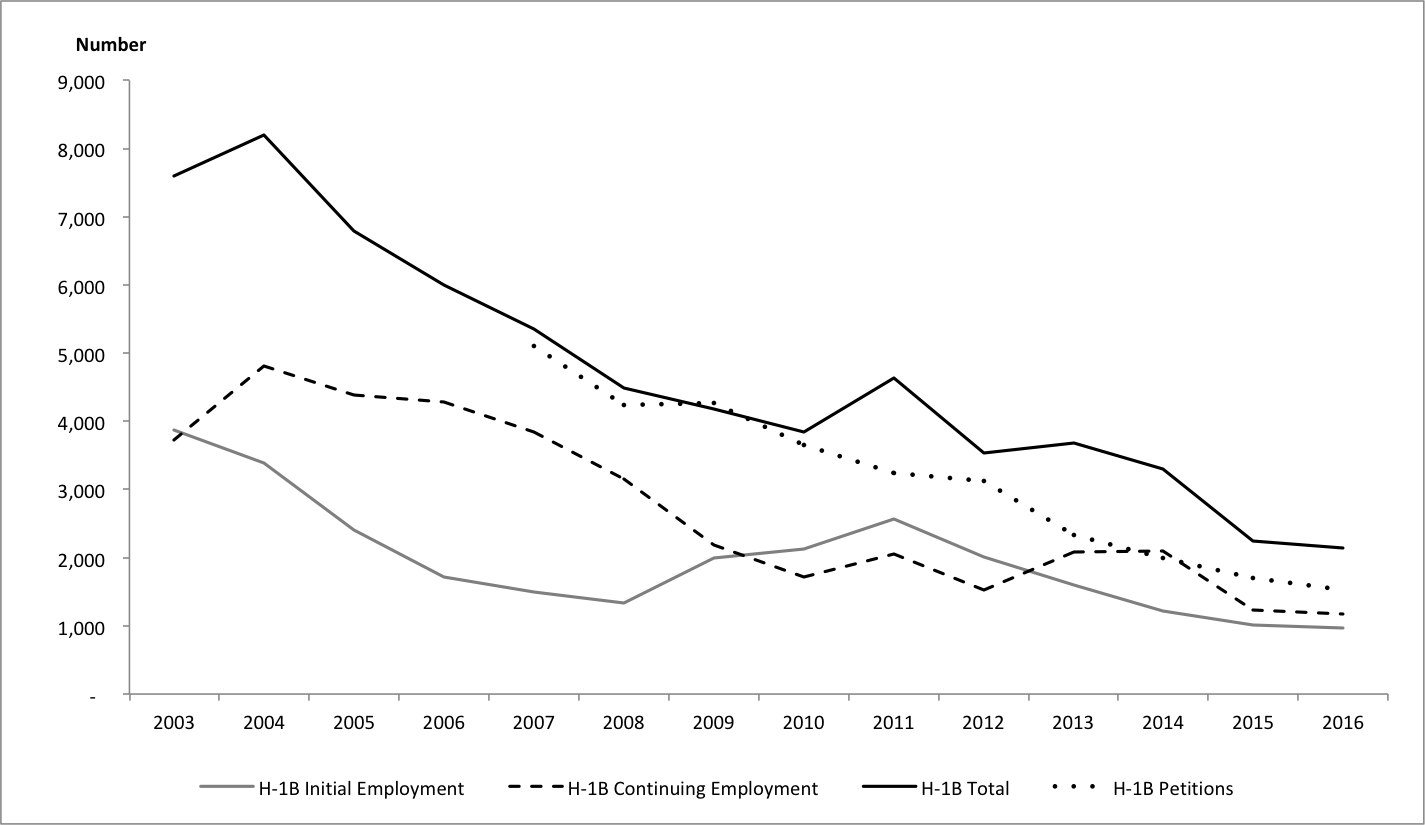
\includegraphics[scale=0.5]{H-1B_UK.png}
\caption{H-1B visa petitions and approvals for UK citizens in the USA, FY 2003-2016. Source: \cite{USCIS2017} and Annual USCIS Reports to Congress}\label{fig:migration}
\end{center}
\end{figure}

There is a high demand in most developed economies for high-skilled immigration to fill skill shortages \citep{Chaloff2009}. While the US has historically attracted a large proportion of the world's highly skilled migrants, other countries, such as Australia and Canada, have increasingly tried to replace the US by enacting immigration policies favoring the highly skilled \citep{Betts2011,Czaika2017,Karaca2018}. More than 120,000 British citizens have emigrated in the year following the Brexit referendum in June 2016; the US has been a favorite destination for high-skilled UK labor emigrants, alongside Australia and Western Europe \citep{ONS2017}.
%\footnote{Around 70,000 British citizens immigrated to the UK, resulting in net emigration of 50,000.} 
However, the attractiveness of the US seems to be in decline, as indicated by fewer H-1B visa petitions for UK high-skilled workers (Figure \ref{fig:migration}).\note{The H-1B visa is employer-sponsored and the largest visa program for temporary skilled immigration to the US. For an overview of the program see \cite{Kerr2010}.}  We provide insights into these trends by implementing an experiment designed to explore the factors shaping the demand (on the part of skilled potential emigrants) for migration destinations. %This trend could potentially be reversed post-Brexit by stronger ties between the UK and the USA, resulting in increased migration.


\paragraph{Social Welfare.} There is mixed evidence suggesting that emigration decisions of high-skilled individuals are determined by social welfare policies, such as after-tax wages, the wage premium for education, welfare benefits, and health and education systems. \citep{Boeri2012,Czaika2017,Geis2013}.\note{Policies to facilitate or restrict emigration could also affect migration decisions but have received little academic attention \citep{McKenzie2013}.}  For example, \citet{DeGiorgi2009,Boeri2010} and \cite{Borjas1999} find that generous welfare states attract more (and predominantly lower skilled) immigrants.  However, \citet{Giulietti2013} conclude that there is no significant relationship between welfare and immigration. 
%Further, non-economic factors, such as migrant networks, family, and friends affect emigration decisions \citep{Boyd1989,Garip2008}. [DL: CONSTANTIN, WHY IS THIS RELEVANT FOR THE READER, PLEASE ADD SOME REFERENCE TO OUR STUDY] 
%[CR: I included non-economic factors, as they are generally seen as important in migration decision making. however, as we do not include them in the empirical analysis, we might be able to cut them?] 

\paragraph{The politics of emigration decisions.} 
Other aspects that potentially shape emigration decisions are social attitudes and the political discourse around immigration in the destination country. Assuming equal socio-economic benefits from migration, migrants would presumably relocate to a country where they feel welcome rather than to one where they are greeted with hostility. 

\par President Trump seems to be shutting the door to (high-skilled) immigration, despite individual attitudes in the US in favor of high-skilled immigration \citep{Iyengar2013, Valentino2017}; a widening gap between demand and supply of skilled labor \citep{Chaloff2009}; and job openings at record high levels and low unemployment \citep{Desilver2017}. Strict immigration policies, alongside political populism, nativism, anti-immigrant rhetoric, and xenophobia might deter or deflect the highly skilled \citep{Czaika2017b}. %The ``Trump effect'' could therefore potentially partly explain the decreasing attractiveness of the USA for high skilled UK emigrants. 

%\par There is a high demand in most developed economies for high skilled immigration \citep{Chaloff2009}. This is due to at least four factors at both the macro and micro level. First, skilled immigration has been shown to have a positive net fiscal impact, i.e. migrants pay more in taxes than they receive in transfers and benefits \citep{OECD2014}. Second, skilled migrants tend to be younger and more educated than the population average of the receiving country, thereby relieving pressure on welfare states and deferring the demographic change, particularly in Europe \citep{Gagnon2014}. Third, skilled migrants disproportionately engage in research, innovation, and entrepreneurship, thereby contributing to economic growth \citep{Hunt2010,Kerr2010,Wadhwa2009}. Fourth, at the micro level, skilled migration helps to meet the rising demand of employers for skilled workers \citep{Chaloff2009}. Technological change, artificial intelligence, digitalization, and automation will further fuel this demand and widen the gap between the supply and demand of domestic skilled workers in many developed countries. %Firms will want to hire foreign high skilled workers for the latter two reasons: their contribution to innovation and the limited supply of domestic high skilled labor.

%\par High skilled immigration generally has a positive net fiscal impact \citep{OECD2014}; relieves pressure on welfare states and defers the demographic change \citep{Gagnon2014}; and contributes disproportionately to research, innovation, and entrepreneurship \citep{Hunt2010,Kerr2010,Wadhwa2009}. 

\par Nativism, ``an ideology, which holds that states should be inhabited exclusively by members of the native group (the nation) and that non-native elements (persons and ideas) are fundamentally threatening to the homogeneous nation-state'' \citep[p.2]{Mudde2012} 
%or as ``intense opposition to an internal minority on the grounds of its foreign (i.e., `un-American') connections'' \cite[p.4]{Higham2002}
has been on the rise in the US \citep{Wadhwa2009}. %\cite{Mudde2012} argues that there are five anti-immigrant nativist frames: cultural, religious, security, economic, and political. 
The `Muslim ban' -- immigration restrictions for Muslim-majority countries; defamations of Hispanics and African Americans as criminals and rapists; the claim that immigrants take American jobs; that Mexico is sending their criminals to the US; and Trump's alleged dismissal of Haiti, El Salvador, and African nations as ``shithole countries'' are all examples of nativist frames in contemporary US discourse. %, Trump's policy changes, announcements thereof, speeches, and tweets 
%\citep{Mudde2012,Fleming2018}. 

\par This anti-immigrant discourse is clearly not aimed at high-skilled UK emigrants.  Our contention is that, nevertheless, this intolerant rhetoric creates a general perception of hostility towards immigrants, irrespective of their country of origin. %Despite a lack of academic studies on the impact of nativism on foreign high skilled potential immigrants, 
There are signs that the `Trump effect' has already led to decreased interest in American jobs from foreign high-skilled individuals \citep{Murnane2017}. Although the British continue to have a favorable view of the US, 
%-- in contrast to the German, French, or Spanish --
the majority have negative views about Trump and his policies \citep{DeVries2018,Wike2017}. %For instance, 83 per cent of respondents from the UK oppose the USA-Mexico border wall and 58 per cent disapprove of the ``Muslim ban'' \citep{Wike2017}. 
These findings further indicate that individuals from countries with higher average skill levels, the young, those on the political left, and women are more critical of Trump's policies. The `Trump effect' might therefore particularly discourage young female leftist high-skilled UK emigrants from relocating to the US.

\par Populism and nativism might not only deter foreign high-skilled immigration, they might also encourage foreign high-skilled workers already in the destination country to emigrate. There are signs that `Trumpian' immigration policies have contributed to high-skilled individuals' intentions to leave the USA \citep{Wadhwa2009}. 

%There are parallels between Trump and Brexit in that immigration was a key salient issue \citep{Goodwin2017}. The `Brexit effect' could therefore discourage foreign high skilled immigration and encourage emigration of foreign high skilled workers from the UK \citep{Jack2018}. The statistics provide evidence for both conjectures: a fall in net migration, driven by less immigration from the EU and more emigration of EU citizens; a drop of applications from EU nationals for undergraduate study in the UK; a decrease in the attractiveness of the UK labor market for high-skilled graduates from the EU; and almost 10,000 EU health workers have quit the NHS since the Brexit vote, an increase of 22 per cent on 2016 and 42 per cent on 2015 \citep{Busse2017,ONS2017,Walker2017}.
 
%and cultural values, demographic factors, and ideology played a central role for people supporting Trump and Brexit \citep{Inglehart2016}.
%More than 100,000 EU citizens have left the UK in the year following Brexit, the majority for work-related reasons \citep{ONS2017}. 
 %Further, British nativism  might even encourage high skilled UK  citizens to emigrate amid the increasing number of hate-crime reports, intolerance, and xenophobia \citep{Dearden2017a,Dearden2017b}.

%The shaded area represents the number of individuals whose H-1B petition was approved but who have not been successful in securing a visa. 

%\begin{figure}
%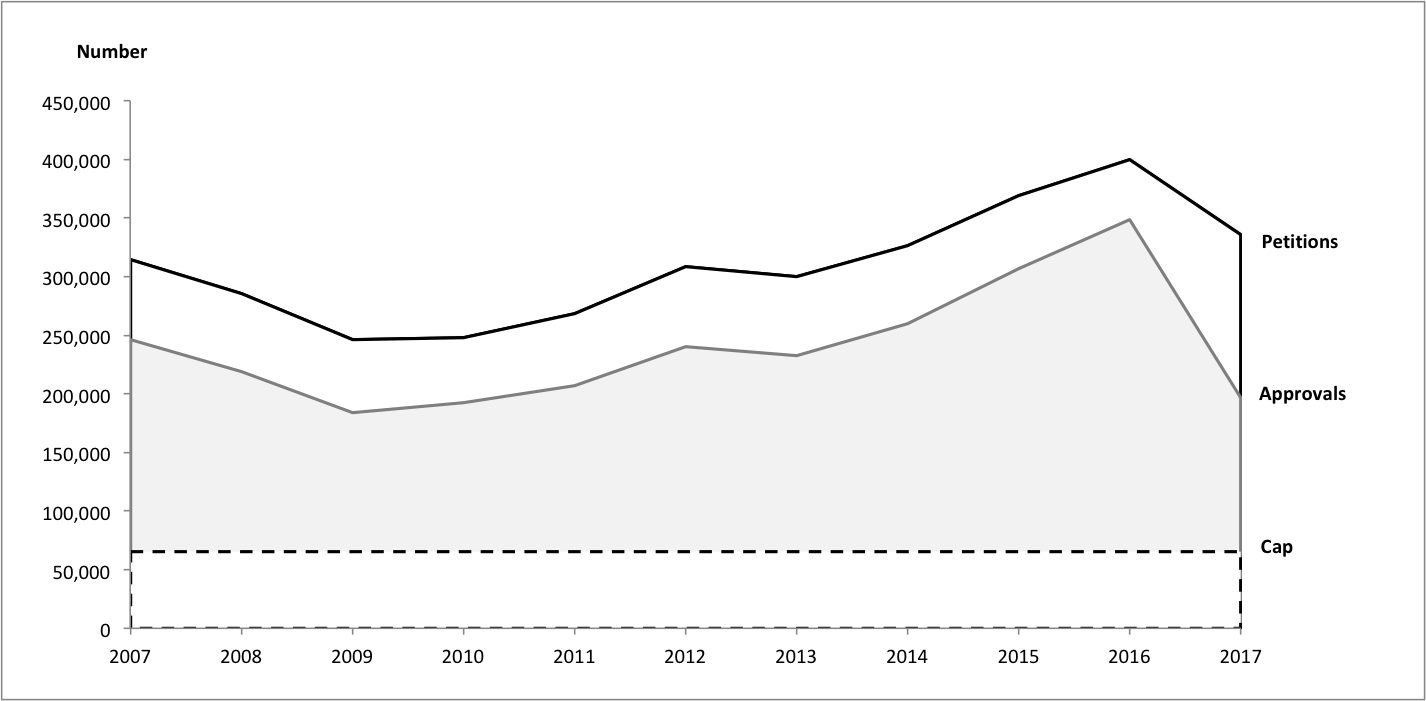
\includegraphics[width=\textwidth]{H-1B.png}
%\caption{H-1B visa petitions, USA FY 2007-2017. Source: \cite{USCIS2017}}
%\end{figure}

%\par Nativism likely also affects USA employers' demands for foreign high skilled workers due to increasing complexity of visa policies and uncertainty over Trump's ``America first'' policies \citep{Murnane2017}. A concrete sign of the increasing reluctance to hire foreign high skilled labor is the 16 per cent decrease in H-1B petitions\note{For comparison, H-1B petitions have increased by seven per cent on average since 2009.}; a sign for the growing visa restrictiveness is the 43 per cent drop in approvals for H-1B petitions in 2017 \citep{USCIS2017}. Similarly, British employers might be less likely to hire EU nationals amid uncertainty over future post-Brexit regulations \citep{CIPD2017}.

\par Having highlighted early signs that nativism and populism might have a detrimental effect on the preferences of foreign high-skilled labor to immigrate to the USA, we aim to causally identify their effect -- as well as the effect of classic migration drivers -- on emigration preferences of high-skilled UK citizens. We make two contributions. First, a novel quantitative measure of the importance of different migration drivers, including salary, welfare benefits, education opportunities, nativist immigration policies, and the destination country itself. Second, our findings could help to inform post-Brexit immigration policy and give insight into future migration flows between the US and the UK. We summarise our conjectures below.

\paragraph{Politics: Nativist Policy Cues.} Our core contribution is to isolate the causal effect of strident anti-immigration rhetoric and policies on the migration decisions of highly skilled potential immigrants. Given the above discussion we expect that:

\begin{enumerate}

\item The US may no longer be the only (or the most) preferred destination for high-skilled foreign individuals. High-skilled UK citizens might increasingly prefer to relocate to Australia or Canada;

\item Associating ``US'' with skilled job offers significantly reduces their appeal to prospective employees in highly skilled foreign labor pools;

\item Associating `Trumpian' immigration policies with skilled job offers significantly reduces their appeal to prospective employees in highly skilled foreign labor pools; and,

\item These effects are stronger for high-skilled UK citizens with less favorable views of the US and who are more critical of Trump's policies (e.g. those on the political left, the young, and women).


\end{enumerate}

\paragraph{Socio-economic conditions shaping migration decisions.} As pointed out earlier, there are also socio-economic characteristics of destination countries that make them more, or less, attractive to migrants. Our estimation strategy will allow us to assess the extent to which these factors, compared to the nativist policy signals described above, shape the migration decision. Our conjectures are the following:  

\begin{enumerate}
\setcounter{enumi}{4}
\item Economic self-interest should certainly play a role in the emigration decision. Countries with higher average salaries are expected to be more appealing; as are countries that have experienced above average rates of GDP growth.  Higher levels of economic growth should signal greater prospects for suitable employment.  And since our focus is on high-skilled potential U.K. emigrants, the expectation is that levels of salaries in the service sector would be of particular interest.

\item The generosity of country's welfare benefits can be a positive signal for many potential migrants, particularly those emigrating from countries with a generous welfare state.  Government policies, such as a guaranteed monthly family allowance and a generous minimum wage, may significantly increase a country's appeal to prospective employees in highly skilled foreign labor pools.  While it is true that these high-skilled UK migrants will not benefit from these welfare policies, we know that they receive strong support from a large majority of the U.K. population and particularly from the highly skilled and educated segments of society \citep{Heathetal1994}.

\item High-skilled emigrants are expected to give considerable weight to the quality of the education infrastructure in the countries to which they are considering migrating.  Countries that rank at the top of the international league tables for education, such as is the case for US universities, should weigh significantly in the migration decisions of high-skilled potential migrants.

\end{enumerate}

%\item If liberal and social media reflects accurate social preferences, the Muslim ban should have a negative effect on migration preferences, even if other traits (economic growth and social benefits) are better in that country than in the alternative country.   

%\item If social benefits are driving decisions, then it should have a positive effect on migration preferences, even when economic conditions (growth and/or salaries) are not as strong in the other destination. 

%\item There might be a socio-economic interaction effect here, with a stronger effect of social benefits among people that are most likely to be beneficiaries of social benefits (lower levels of income), but this effect may be small in student subject pools. 
% -- CR: if we have high skilled foreign labor pools, I do not think we will have an interaction effect. should we therefore bother to include it?

%\item For social benefit variables to have a lower impact on migration preferences for high ability types than low ability types. 

%\item I would expect the coefficient for economic growth and salary percentile to have a larger impact on migration preferences for high ability types than low ability types. 
% -- CR: how do we measure high and low ability types?

\section*{Experiment Design}

\par Our intuition is that highly skilled potential emigrants from the UK will seek out, and be exposed to, various characteristics of destination countries. And again our intuition here is that the messages that resonate will be primarily economic and political. We focus on three economic characteristics: welfare benefits, educational opportunities, and salary levels. With respect to politics, we are interested in whether strident anti-immigrant messages play a relatively important causal role in forming emigration preferences compared to the other salient information potential migrants acquire. We believe that conjoint survey experiments might be ideal for teasing out the causal effect of this strident anti-immigrant rhetoric.  
\par The power of conjoint survey experiments for identifying the causal effect of different choice attributes has been extensively developed in political science \citep{Hainmuelleretal2013,Hainmuelleretal2015}. But of course conjoint experiments have a long history and have been widely implemented in the social sciences.   

\par Our conjoint design has the following features: Subjects choose between Employment Destination 1 and Employment Destination 2 (those exact choice names are provided). Each employment destination has five attributes and each attribute has three values. The values associated with each attribute are randomly assigned to each of the two destinations for each choice set presented to the subjects. There are three conjoint experiments, which vary the attributes displayed to the participant. Subjects make three choices per conjoint, for a total of nine choices. The five attributes of the conjoint design correspond to the factors we conjectured drive the migration decision for skilled labor. Table~\ref{tab:attributes} summarizes the attributes and their values. Screenshots of the conjoint treatments are presented in the online appendix.

\begin{table}[!ht]
\caption{Immigration Conjoint Experiment Treatments}\label{tab:attributes}
\begin{center}
\begin{tabular}{lccc}\footnotesize
&\bf Conjoint& \bf Conjoint& \bf Conjoint\\
&\bf  1 & \bf  2 & \bf  3 \\
\hline\hline
\bf Social Benefits &  & & \\
Generous guaranteed& Yes & Yes & Yes \\
monthly family allowance (+)&  &  &  \\
Basic hourly minimum wage (neutral)& Yes & Yes  & Yes \\
No state minimum wage or income support (-)& Yes & Yes & Yes  \\
\hline\hline
\bf Economy  &  & & \\
Annual GDP Growth of 6 percent (+)& Yes & Yes & Yes \\
Annual GDP Growth of 4 percent (neutral)& Yes & Yes  & Yes \\
Annual GDP Growth of 2 percent (-)& Yes & Yes & Yes  \\
\hline\hline
\bf Education (Average international rank)      & & & \\
Universities: 90th Percentile (+)& Yes & Yes & Yes \\
Universities: 60th Percentile (neutral)& Yes & Yes  & Yes \\
Universities: 40th Percentile (-)& Yes & Yes & Yes  \\
\hline\hline
\bf Service Jobs (Average international rank)  & & & \\
Service salaries: 90th Percentile (+)& Yes & Yes & Yes \\
Service salaries: 70th Percentile (neutral)& Yes & Yes  & Yes \\
Service salaries: 50th Percentile (-)& Yes & Yes & Yes  \\
\hline\hline
\bf Immigration One   & & & \\
  Implementation of point-system (positive) (+)& Yes & No & No \\
Change in visa processing centres (neutral)& Yes & No  & No \\
 Restriction on Muslim & Yes & No & No  \\
immigration/tourist visas (-)&  &  &   \\
\hline\hline
\bf Immigration Two   & & & \\
  Implementation of point-system (positive) (+)& No & Yes & No \\
Change in visa processing centres (neutral)& No & Yes  & No \\
  Deportation of all illegal immigrants (-)& No & Yes & No  \\
\hline\hline
\bf Country    &  & & \\
USA (-)& No & No & Yes \\
Australia (neutral)& No & No  & Yes \\
Canada (+)& No & No & Yes  \\
                  \hline\hline
\end{tabular}
\end{center}
\end{table}

%\clearpage

\par We have implemented different immigration treatments to tease out the immigration rhetoric, or simple country cues, that might cause potential high skilled immigrants to avoid migrating to specific destination countries. There are four treatments designed to capture the classic factors that might affect emigration preferences of high-skilled labor: social benefits, the economy, education opportunities, and the attractiveness of service sector jobs. These treatments are implemented in all three conjoint experiments. There are three different immigration treatments corresponding to the three conjoint experiment columns in Table~\ref{tab:attributes}. The first two conjoint experiments simply vary the nature of the anti-immigration rhetoric or policy. In the third conjoint, we vary the country name -- the idea is that the US `brand' has been sufficiently tarnished by `Trumpian' policies and rhetoric to cause potential highly skilled migrants to avoid the US.

\paragraph{Subject Pool.} The subject pool plays a critical element in our experimental design. Our goal is to identify economic and political factors that could influence high-skilled migration to the US. The subjects in this experiment are drawn from a convenience sample consisting of University of Oxford students who are registered in the Nuffield College Centre for Experimental Social Sciences subject pool.  These students have the high-skilled labor profiles that would be of interest to US firms. Table~\ref{tab:subjects} (online appendix) summarizes the subject profiles for this experiment. The experiments were conducted with Nuffield CESS Online facilities and implemented on Qualtrics. In addition, the experiments were incentivized and offered subjects proper compensation for their time. On average, subjects took 18 minutes and earned \pounds5. All participants are 18 or older, each of them signed a consent form before taking part in the survey, and no deception was used.   

\par Participants in the study are predominantly young (mean age $=26$, standard deviation $=8.6$), as expected with a (current and former) student subject pool that includes post-graduates. Female participants (56 percent) slightly outnumber males. The ideological self-placement of subjects follows a fairly normal distribution, although, as we expected with student subjects, the distribution is skewed to the Left. Participants' interest in migrating is relatively high, with a mean of 5.5 in a 1--7 point scale, indicating the relevance of the subject pool as representatives of potential high-skilled migrants. The self-reported likelihood of emigrating is also high, with a mean of 4.9 in a 1--7 point scale, however, somewhat lower than interest in migration. Including these variables as controls does not alter the results of the estimation (see Table~\ref{tab:results_controls}, online appendix). The full summary statistics (Table~\ref{tab:subjects}) and relevant density plots are available in the online appendix.

\par Overall, participants rated Canada and Australia more favorably than the US ($p<0.000$ and $p = 0.000137$ for pairwise t-tests). This result possibly stems from the slight over-representation of females and those who identify as on the political left in the subject pool. However, the negative evaluation of the US brand persists in the logit estimations that control for age and gender (Table~\ref{tab:results_controls}, online appendix).

\par Balance tests were carried out to evaluate adequate implementation of the randomization protocol (Tables ~\ref{tab:balance1}-\ref{tab:balance5}, online appendix). Multinomial logit estimations of the likelihood of observing a specific attribute indicate that people most interested in migrating were presented the Canada attribute a significantly lower amount of times. Given the importance of having a balanced potential migrant sample across treatments, we included this variable as a control in the estimations. However, it is not a substantive or consistent predictor of destination choice and omitting it does not alter results (data in replication material). Age also has a significant association with the likelihood of observing ``No state minimum wage,'' however, it is not associated with any other of the conjoint attributes and including ``Age'' as a control does not alter the results of the estimations. This could be caused by the existence of a few older participants in the sample. The ``Other'' gender category also appears significant in the balance tests but is because only one person identified as such.

%\par This immigration project focuses exclusively at the high skilled subject pools and accordingly, we used the CESS Oxford student lab pool... a decidedly highly skill sub-group in the UK population.

%In order to do this we administer the experiments with students from post-secondary institutions in the four countries.  And since Nuffield CESS has experimental labs in these four countries were able to exploit their large lab subject pools for the online experiments.  In the UK  we used the CESS Oxford student lab pool; in Chile we recruited students from CESS's University of Santiago Chile subject pool; in China the students were from the CESS subject pools in Wuhan and Nankai Universities; and in India we used the CESS FLAME University subject pool.  This provides us with a unique global pool of subjects who represent the kinds of high skilled talent that U.S. firms are interested in recruiting and hiring.

\section*{Estimation strategy and results}

\par We adopt a very simple strategy for recovering the causal effects of the specific characteristics of emigration destinations: we estimate a logistic regression of destination choice (whether subjects choose or do not choose any of the destination choices) with clustered standard errors at the individual level. Recall that subjects make choices for nine two-destination choice sets -- each subject makes three dichotomous choices for each of the three conjoint treatments. Figure~\ref{fig:treatment_combined} presents graphical summaries of the estimated effects of the regression coefficients with 95 percent confidence intervals -- see the full regression table in the online appendix. The reference categories for the conjoint attributes are the neutral categories indicated in Table~\ref{tab:attributes} and they are included as dots with coefficient zero in Figure~\ref{fig:treatment_combined}.

\begin{figure}%[!t]
\caption{Conjoint Results}\label{fig:treatment_combined}
\centerline{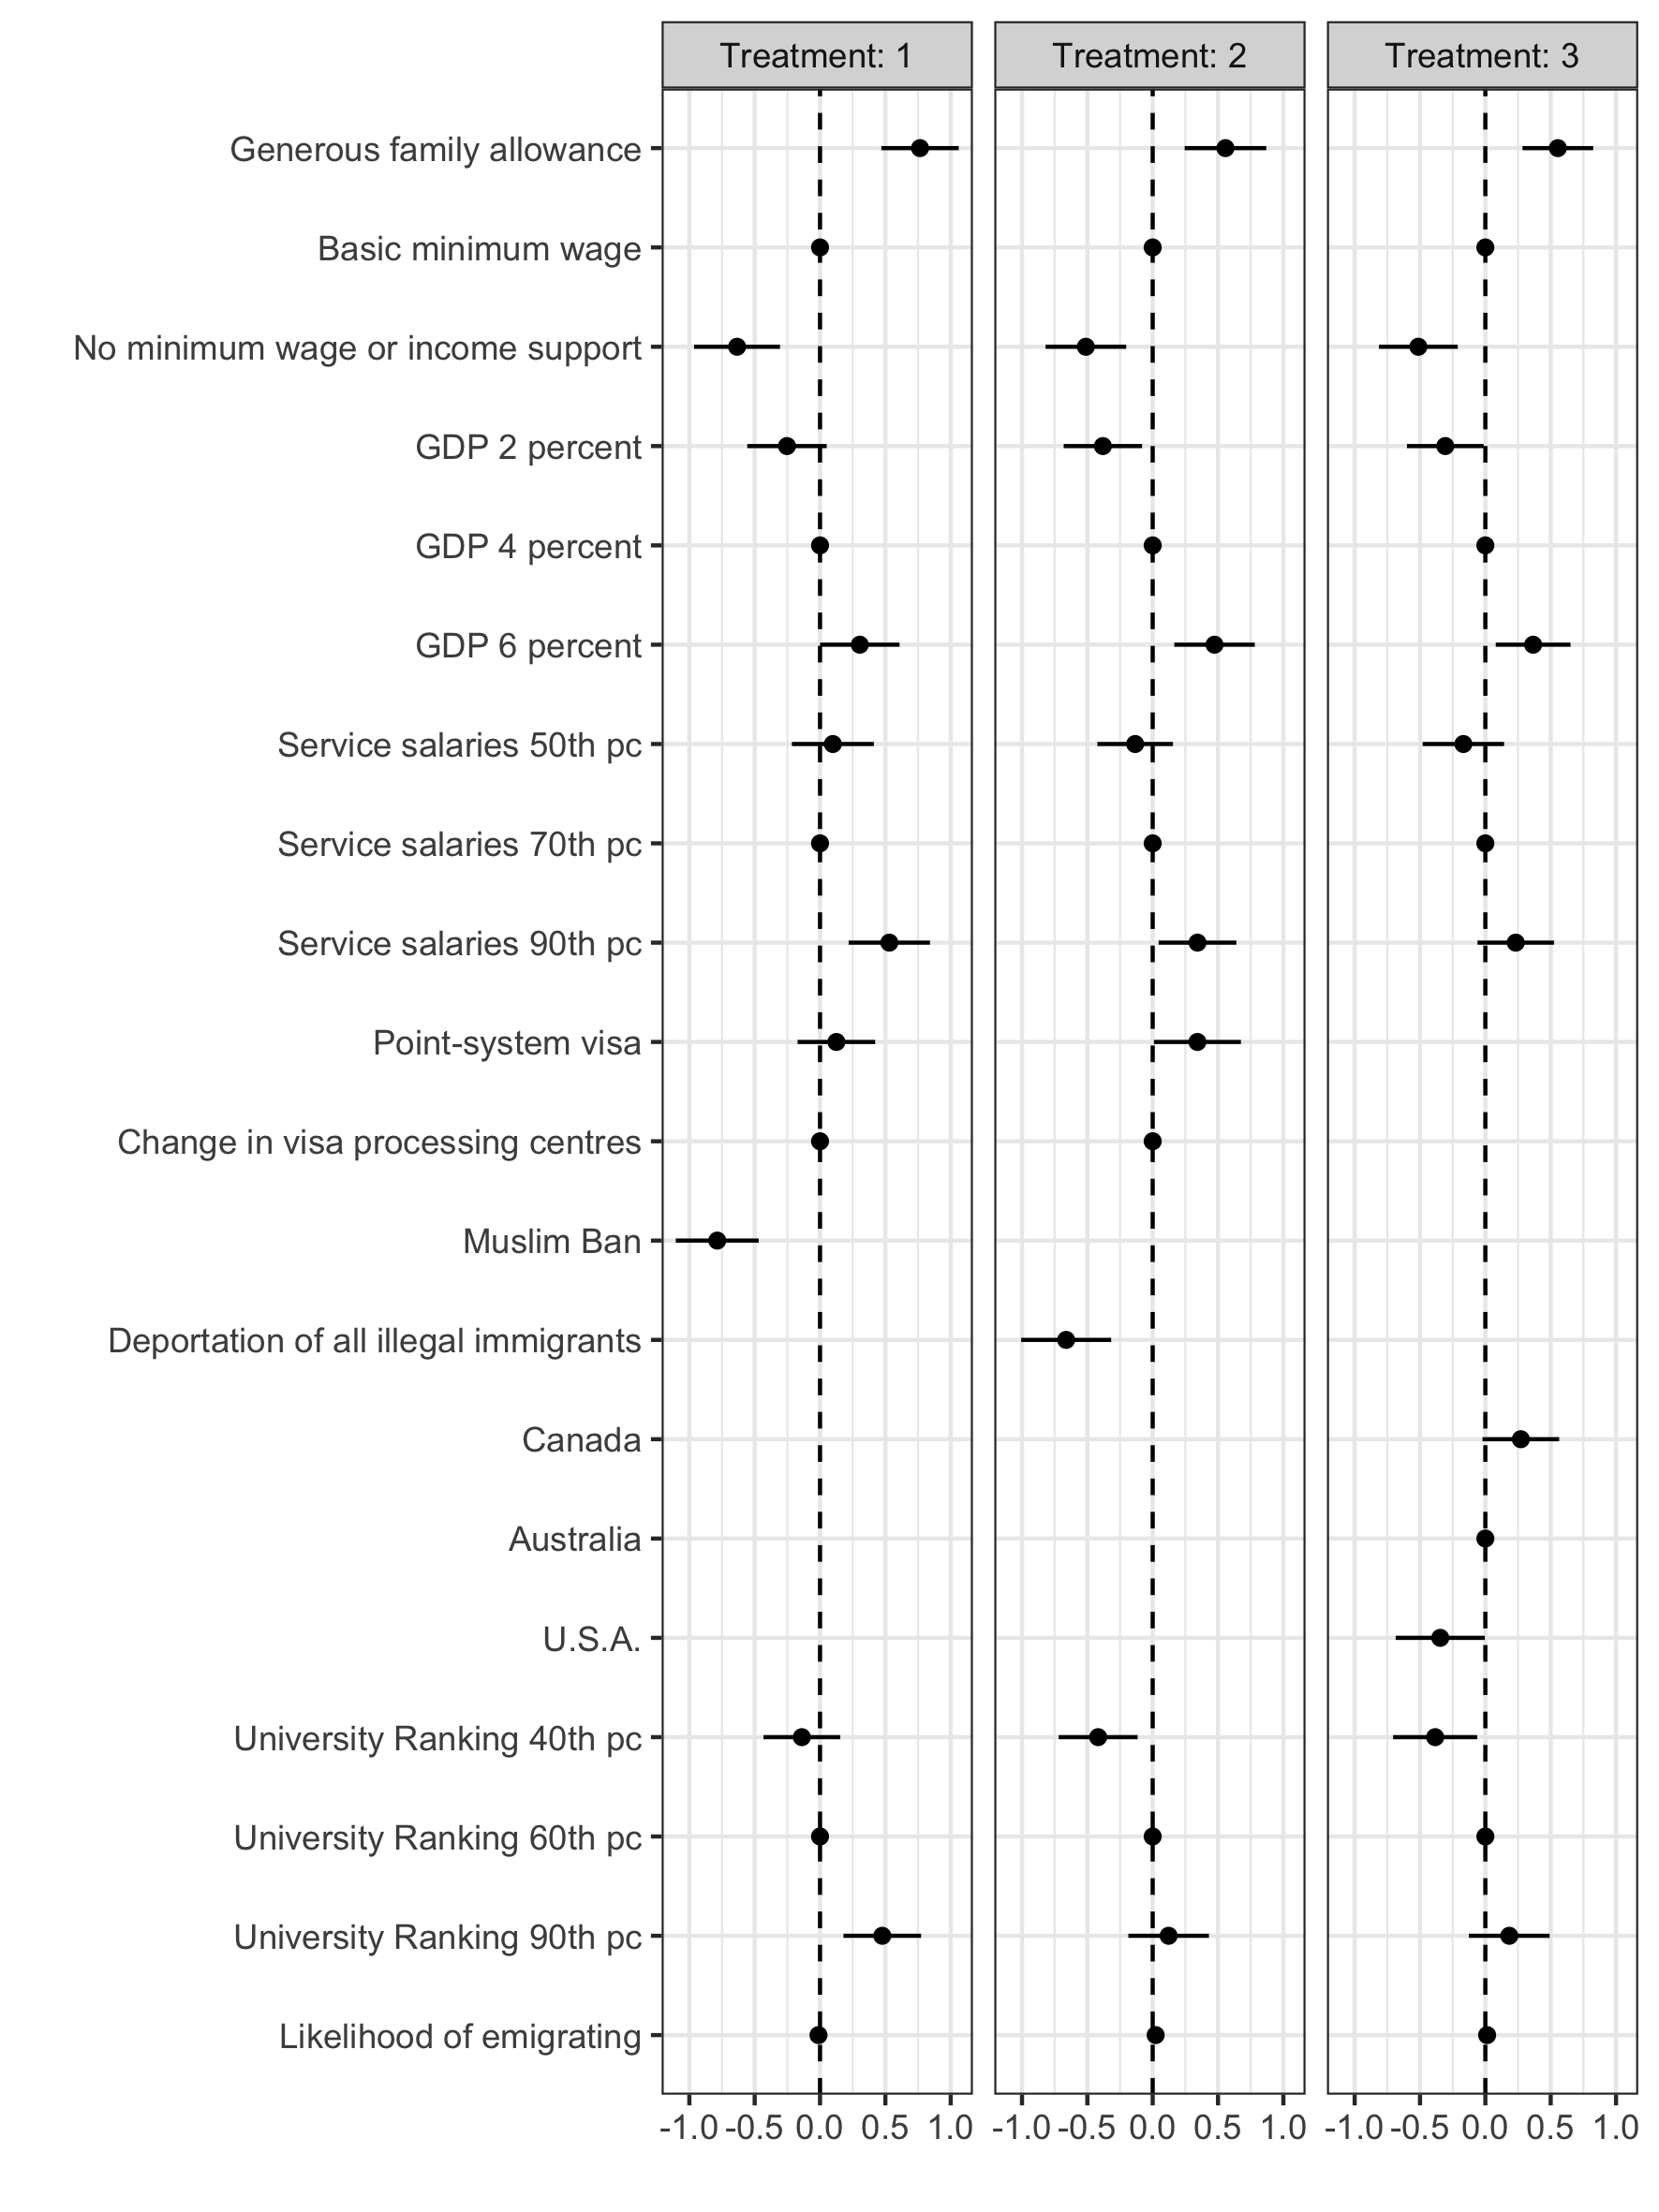
\includegraphics[height=\textheight, width=\textwidth]{conjoint_combined.png}}
\end{figure}



\begin{comment}
\begin{table}[!htbp] \centering 
  \caption{Logistic regression results} 
  \label{tab:results} 
\begin{tabular}{@{\extracolsep{5pt}}lccc} 
\\[-1.8ex]\hline 
\hline \\[-1.8ex] 
 & \multicolumn{3}{c}{Immigration Treatment} \\ 
\cline{2-4} 
\\[-1.8ex] & (1) & (2) & (3)\\ 
\hline \\[-1.8ex] 
 Generous family allowance & 0.765$^{***}$ & 0.557$^{***}$ & 0.555$^{***}$ \\ 
  & (0.151) & (0.159) & (0.138) \\ 
  No minimum wage or income support & $-$0.635$^{***}$ & $-$0.511$^{***}$ & $-$0.513$^{***}$ \\ 
  & (0.168) & (0.157) & (0.154) \\ 
  GDP 2 percent & $-$0.253 & $-$0.381$^{**}$ & $-$0.307$^{**}$ \\ 
  & (0.155) & (0.153) & (0.150) \\ 
  GDP 6 percent & 0.304$^{**}$ & 0.473$^{***}$ & 0.366$^{**}$ \\ 
  & (0.155) & (0.157) & (0.146) \\ 
  Service salaries 50th pc & 0.098 & $-$0.134 & $-$0.168 \\ 
  & (0.160) & (0.148) & (0.159) \\ 
  Service salaries 90th pc & 0.530$^{***}$ & 0.343$^{**}$ & 0.233 \\ 
  & (0.159) & (0.152) & (0.149) \\ 
  Deportation of all illegal immigrants &  & $-$0.662$^{***}$ &  \\ 
  &  & (0.176) &  \\ 
  Point-system visa & 0.125 & 0.342$^{**}$ &  \\ 
  & (0.151) & (0.170) &  \\ 
  Muslim Ban & $-$0.787$^{***}$ &  &  \\ 
  & (0.162) &  &  \\ 
  Canada &  &  & 0.272$^{*}$ \\ 
  &  &  & (0.150) \\ 
  U.S.A. &  &  & $-$0.345$^{**}$ \\ 
  &  &  & (0.174) \\ 
  University Ranking 40th pc & $-$0.139 & $-$0.417$^{***}$ & $-$0.384$^{**}$ \\ 
  & (0.150) & (0.154) & (0.164) \\ 
  University Ranking 90th pc & 0.476$^{***}$ & 0.122 & 0.183 \\ 
  & (0.151) & (0.157) & (0.158) \\ 
  Likelihood of emigrating & $-$0.012 & 0.023$^{*}$ & 0.014 \\ 
  & (0.014) & (0.014) & (0.011) \\ 
  Constant & $-$0.092 & 0.003 & $-$0.019 \\ 
  & (0.213) & (0.199) & (0.201) \\ 
 \hline \\[-1.8ex] 
Observations & 1,170 & 1,170 & 1,170 \\ 
Log Likelihood & $-$731.956 & $-$740.916 & $-$759.410 \\ 
Akaike Inf. Crit. & 1,487.913 & 1,505.832 & 1,542.820 \\   
\hline 
\hline \\[-1.8ex] 
\multicolumn{4}{l}{ \textit{Note:} $^{*}$p$<$0.1; $^{**}$p$<$0.05; $^{***}$p$<$0.01 }  \\ 
\multicolumn{4}{l}{\textit{Standard errors clustered by participant}}
\end{tabular} 
\end{table} 
%\clearpage

\end{comment}

%\par these dummy variables from the equations in Table~\ref{tab:results} help assess the relative importance of these factors on the migration preferences.  Figure~\ref{fig:treatment_one} presents the estimated effect of each attribute value with respect to its referent value. Reference categories are the neutral categories (Table~\ref{tab:attributes}) and Australia, and they are included as dots with coefficient zero

\par The logit results nicely confirm our expectations regarding immigration policy. In the first Immigration Treatment, the ``Muslim Ban'' attribute has a large negative coefficient. In the second Immigration Treatment the ``Deportation'' treatment is negative and large, while the ``Point-system'' treatment is positive. In the third Treatment, the US label has a negative coefficient, indicating a large negative country brand effect (relative to the baseline Australia). 

\par In line with expectations, the destination's economic conditions are relevant. Oxford subjects clearly preferred destinations with higher economic growth and those with higher service sector salaries.  Also as expected, the generosity of social welfare benefits shape migration decisions: the Oxford subjects favor destinations with generous family allowances and they are less attracted by those with no minimum wage or income support. Overall, socio-economic and political factors have a similar effect size on the migration preferences of the highly skilled. In particular, the spread in effect size between the ``No minimum wage/no income support'' value and ``Generous family allowance'' is quite large -- more than the immigration policy effect.

\begin{comment}
\begin{figure}[t!]
\caption{Conjoint Immigration Treatment: Muslim Ban}\label{fig:treatment_one}
\centerline{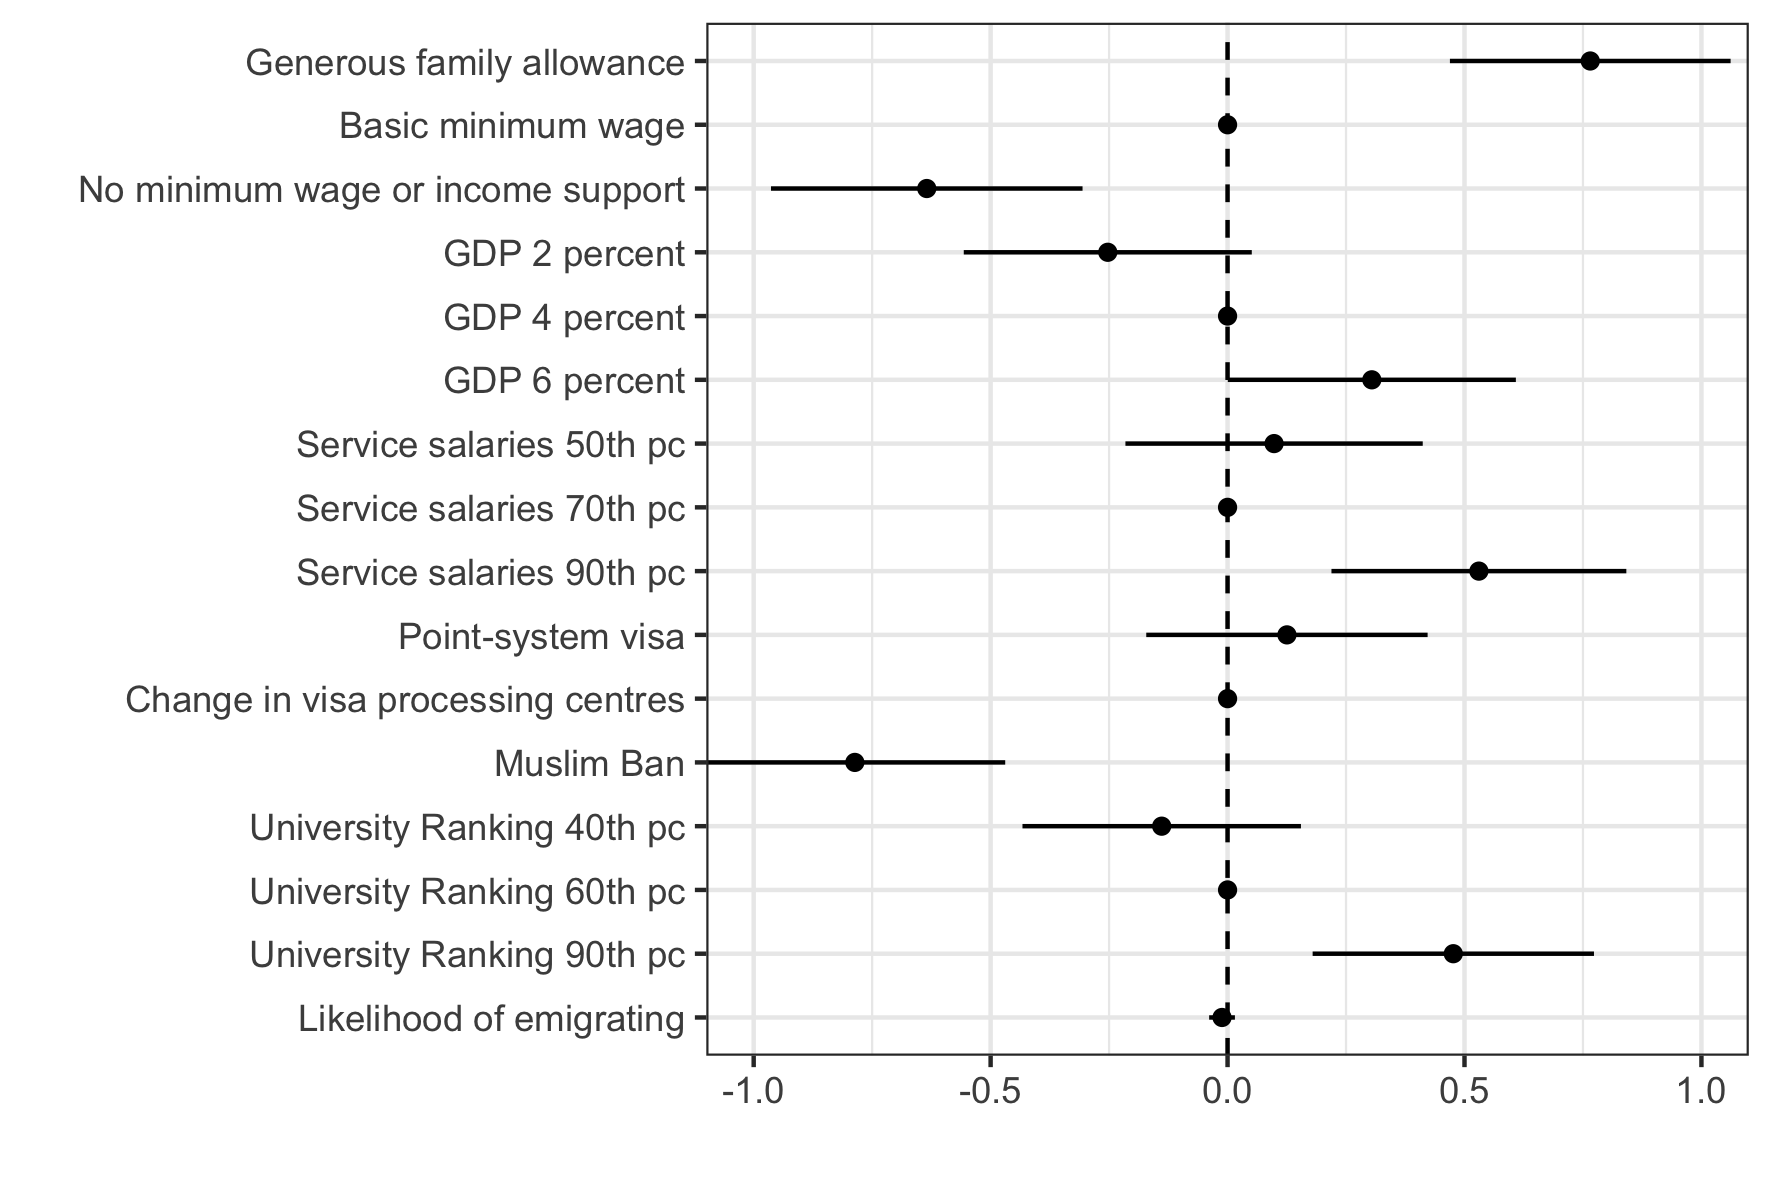
\includegraphics[scale=0.22]{conjoint1.png}}
\end{figure}
\end{comment}

%\par  in Figures \ref{fig:treatment_one}-\ref{fig:treatment_three}. Immigration politics matters and the Muslim Ban Treatment has a large substantive effect (Figure \ref{fig:treatment_one}).  

\begin{comment}
\begin{figure}%[!t]
\caption{Conjoint Immigration Treatment: Deport Illegals}\label{fig:treatment_two}
\centerline{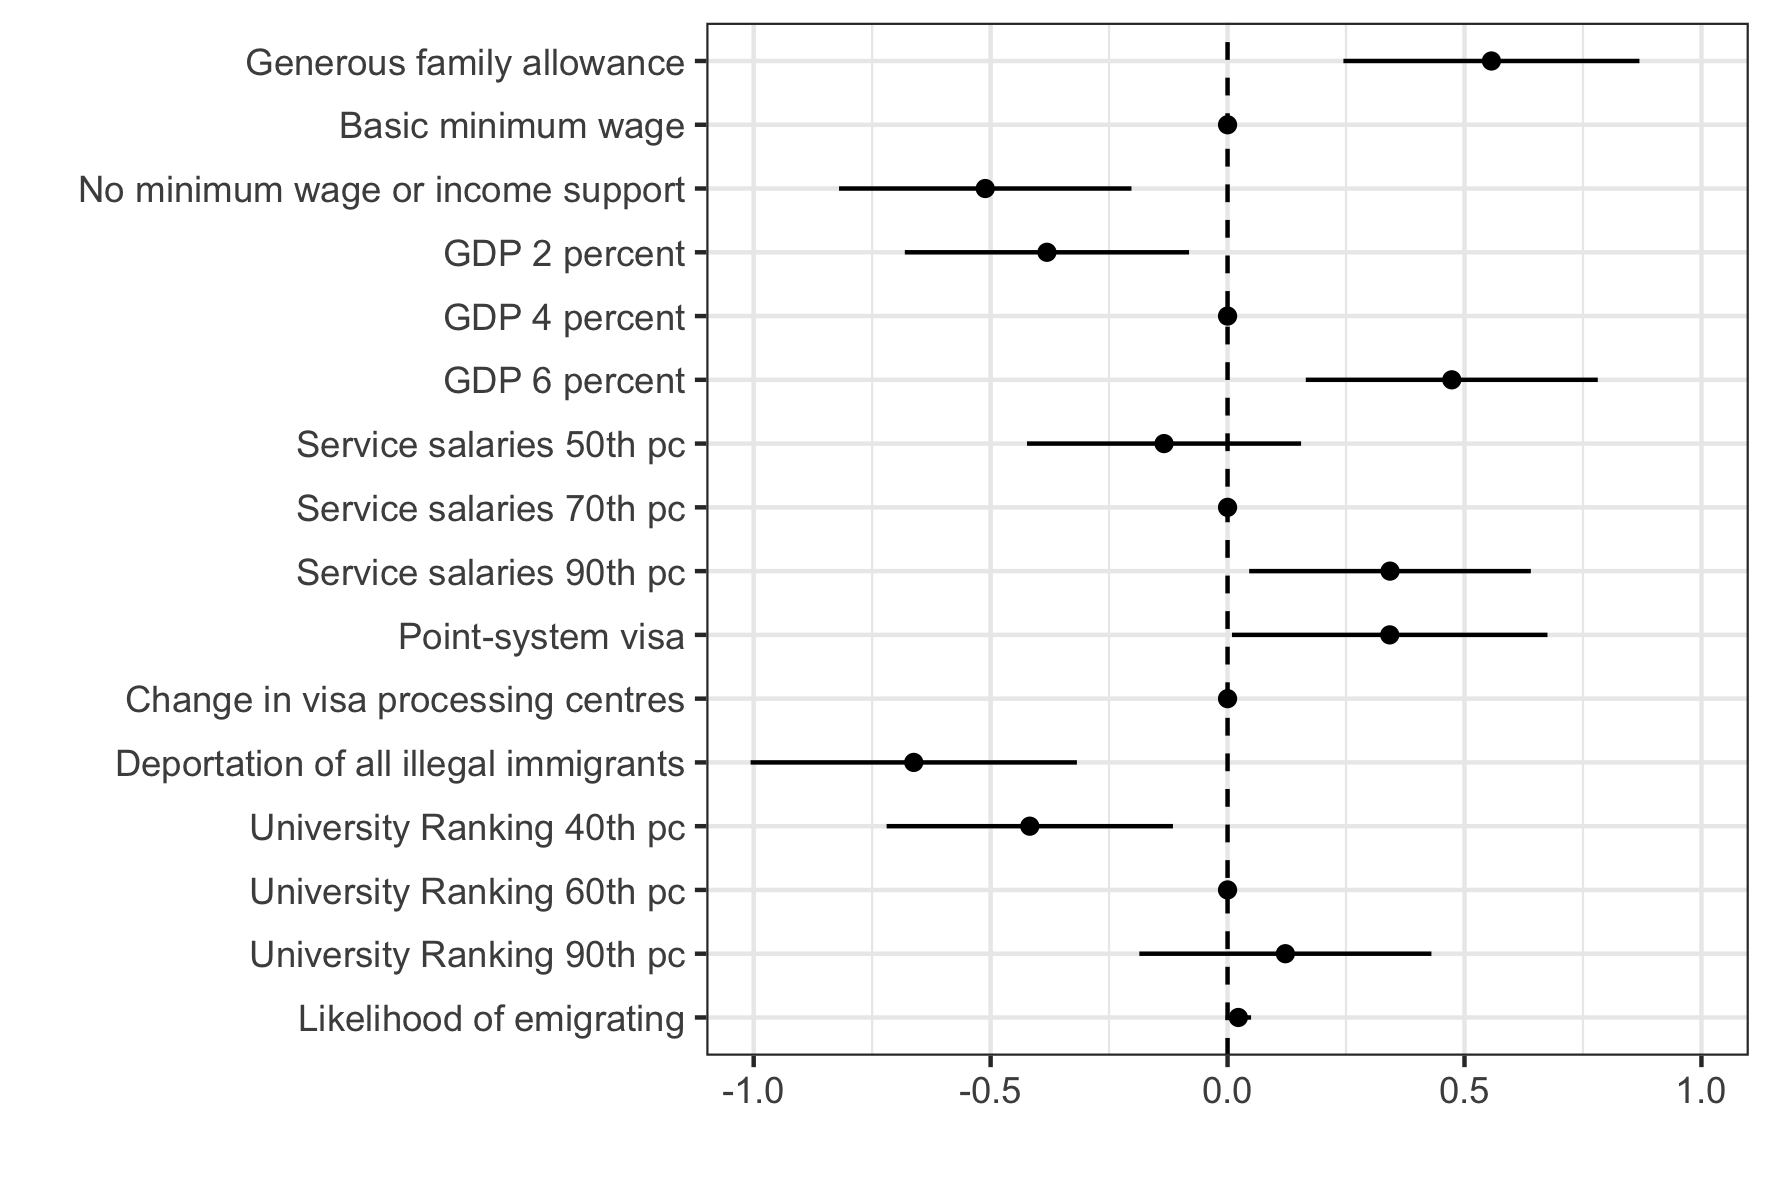
\includegraphics[scale=0.22]{conjoint2.png}}
\end{figure}
%\clearpage
\end{comment}

\par The pattern of effects in the second Immigration Treatment is very similar to Treatment one. Socio-economic factors matter but immigration policy clearly influences migration destination choice. In fact, the spread between the positive ``Point system visa'' and negative ``Deportation of illegal immigrants'' immigration policies is slightly wider than was the case in the first immigration treatment.  

\begin{comment}
\begin{figure}[!t]
\caption{Conjoint Immigration Treatment: Country Names}\label{fig:treatment_three}
\centerline{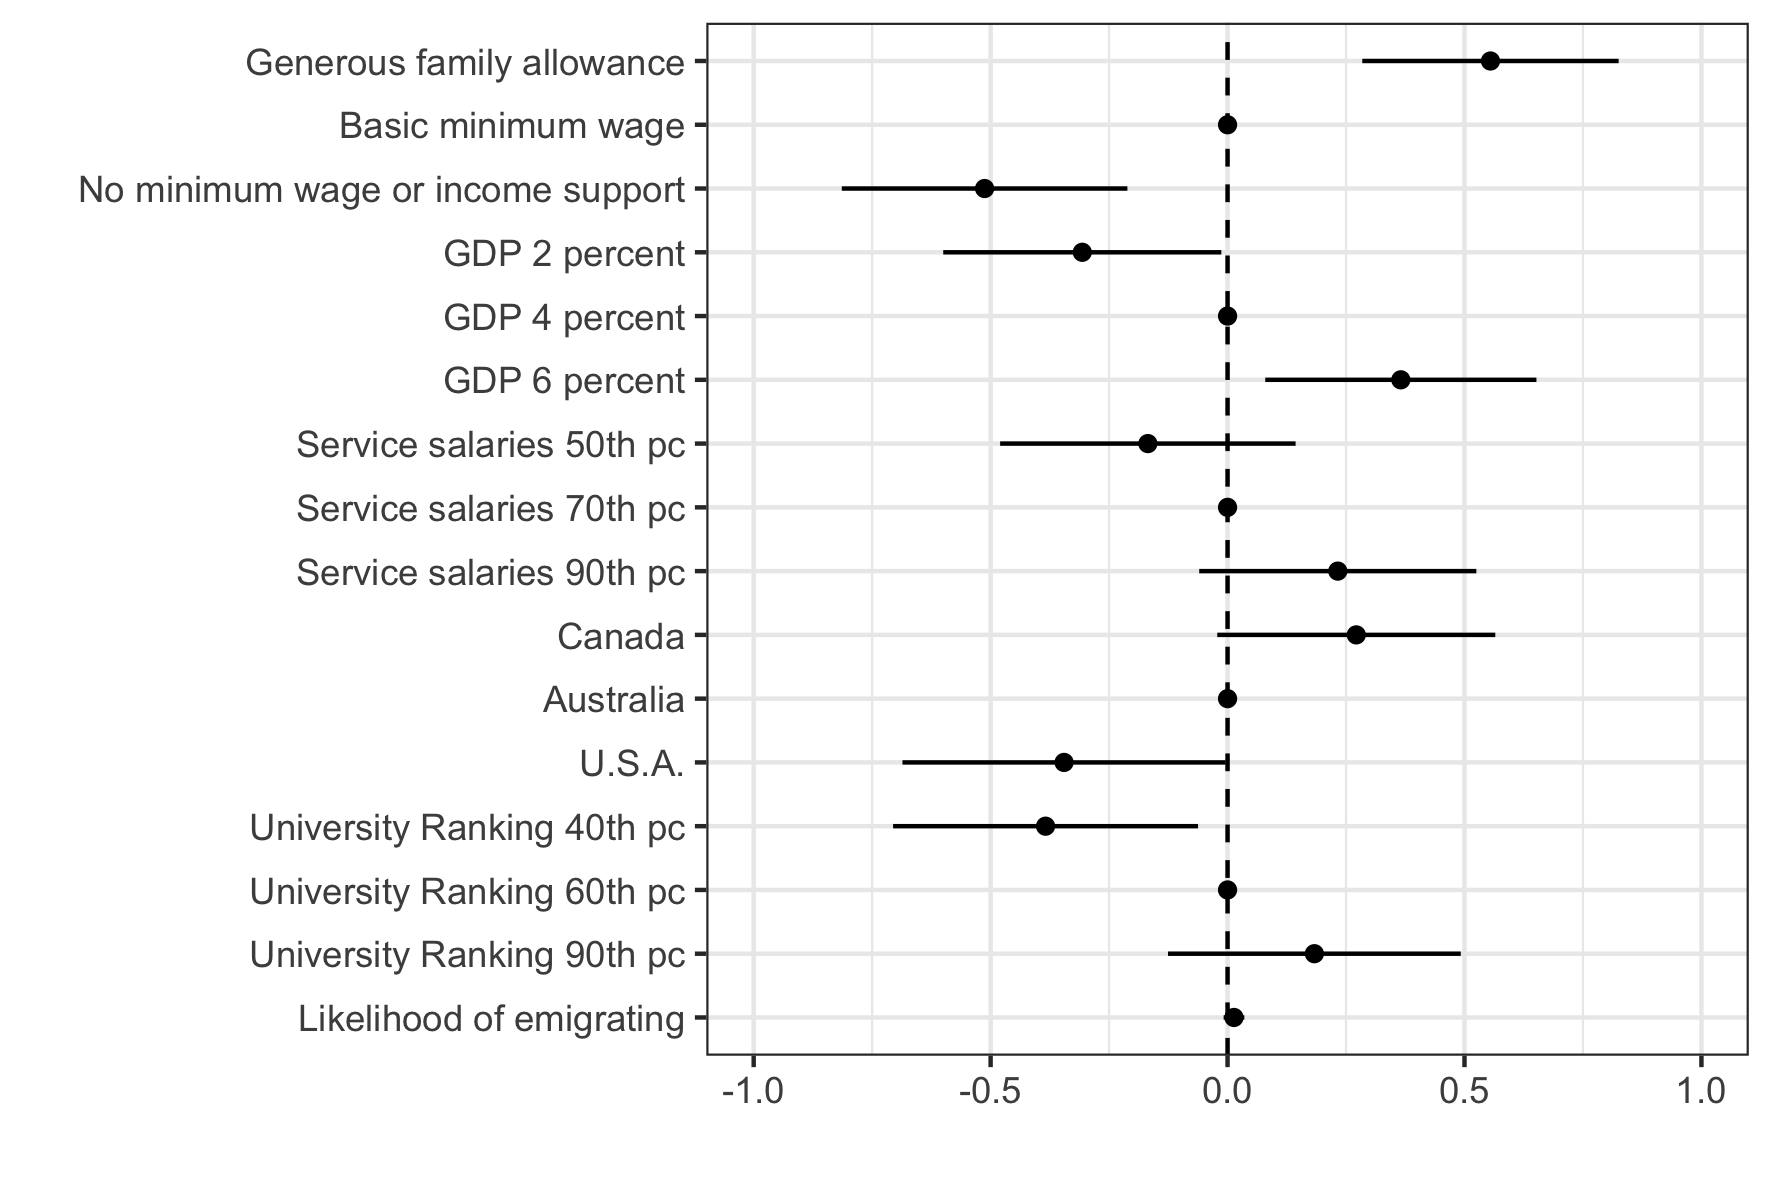
\includegraphics[scale=0.22]{conjoint3.png}}
\end{figure}
\end{comment}

%\clearpage

\par The negative values for the two immigration policy attributes were meant to reflect some of President Trump's nativist rhetoric. Our intuition is that potential high-skilled immigrants to the US are quite informed of this nativist rhetoric and this has tarnished (at least for certain elements of the highly skilled foreign labor pools) the US brand. Our expectation is that we would see exactly the same outcome if we replaced the immigration policy attribute with a country name attribute that included the US as one of the randomly assigned values. The right panel of Figure~\ref{fig:treatment_combined} presents the results from the third immigration treatment.  While the US's political disadvantage is large (coefficient of -0.345), this effect is roughly half of the other politics treatments -- the ``Muslim Ban'' has a coefficient of -0.787, relative to the neutral baseline ``Change in visa processing centres,'' and ``Deportation of illegal immigrants'' has a coefficient of -0.662, relative to the same baseline. These results suggest that while the content of `Trumpian' rhetoric is a strong deterrent for potential UK migrants, the US brand itself does not deter high skilled UK immigrants as much as the specific nativist policies and proposals advocated by President Trump. 


%And the USA effect is smaller than the immigration rhetoric effects in the other two treatments.  The USA brand has a negative effect on the preferences of potential immigrants but the anti-immigration rhetoric has an even more powerful negative effect. 

\par The highly skilled potential UK emigrants that took part in this experiment express a strong and significant preference to migrate to countries with generous social policies.  Certainly with respect to the UK, the US does not have such generous social benefits.  This would represent an additional disadvantage for trying to attract high-skilled migrants to the US (at least for emigrants from the UK.)

%\clearpage

\begin{figure}%[!h]
\caption{Conjoint Treatments: Left-Right Divide}\label{fig:conjoint_ideology}
\centerline{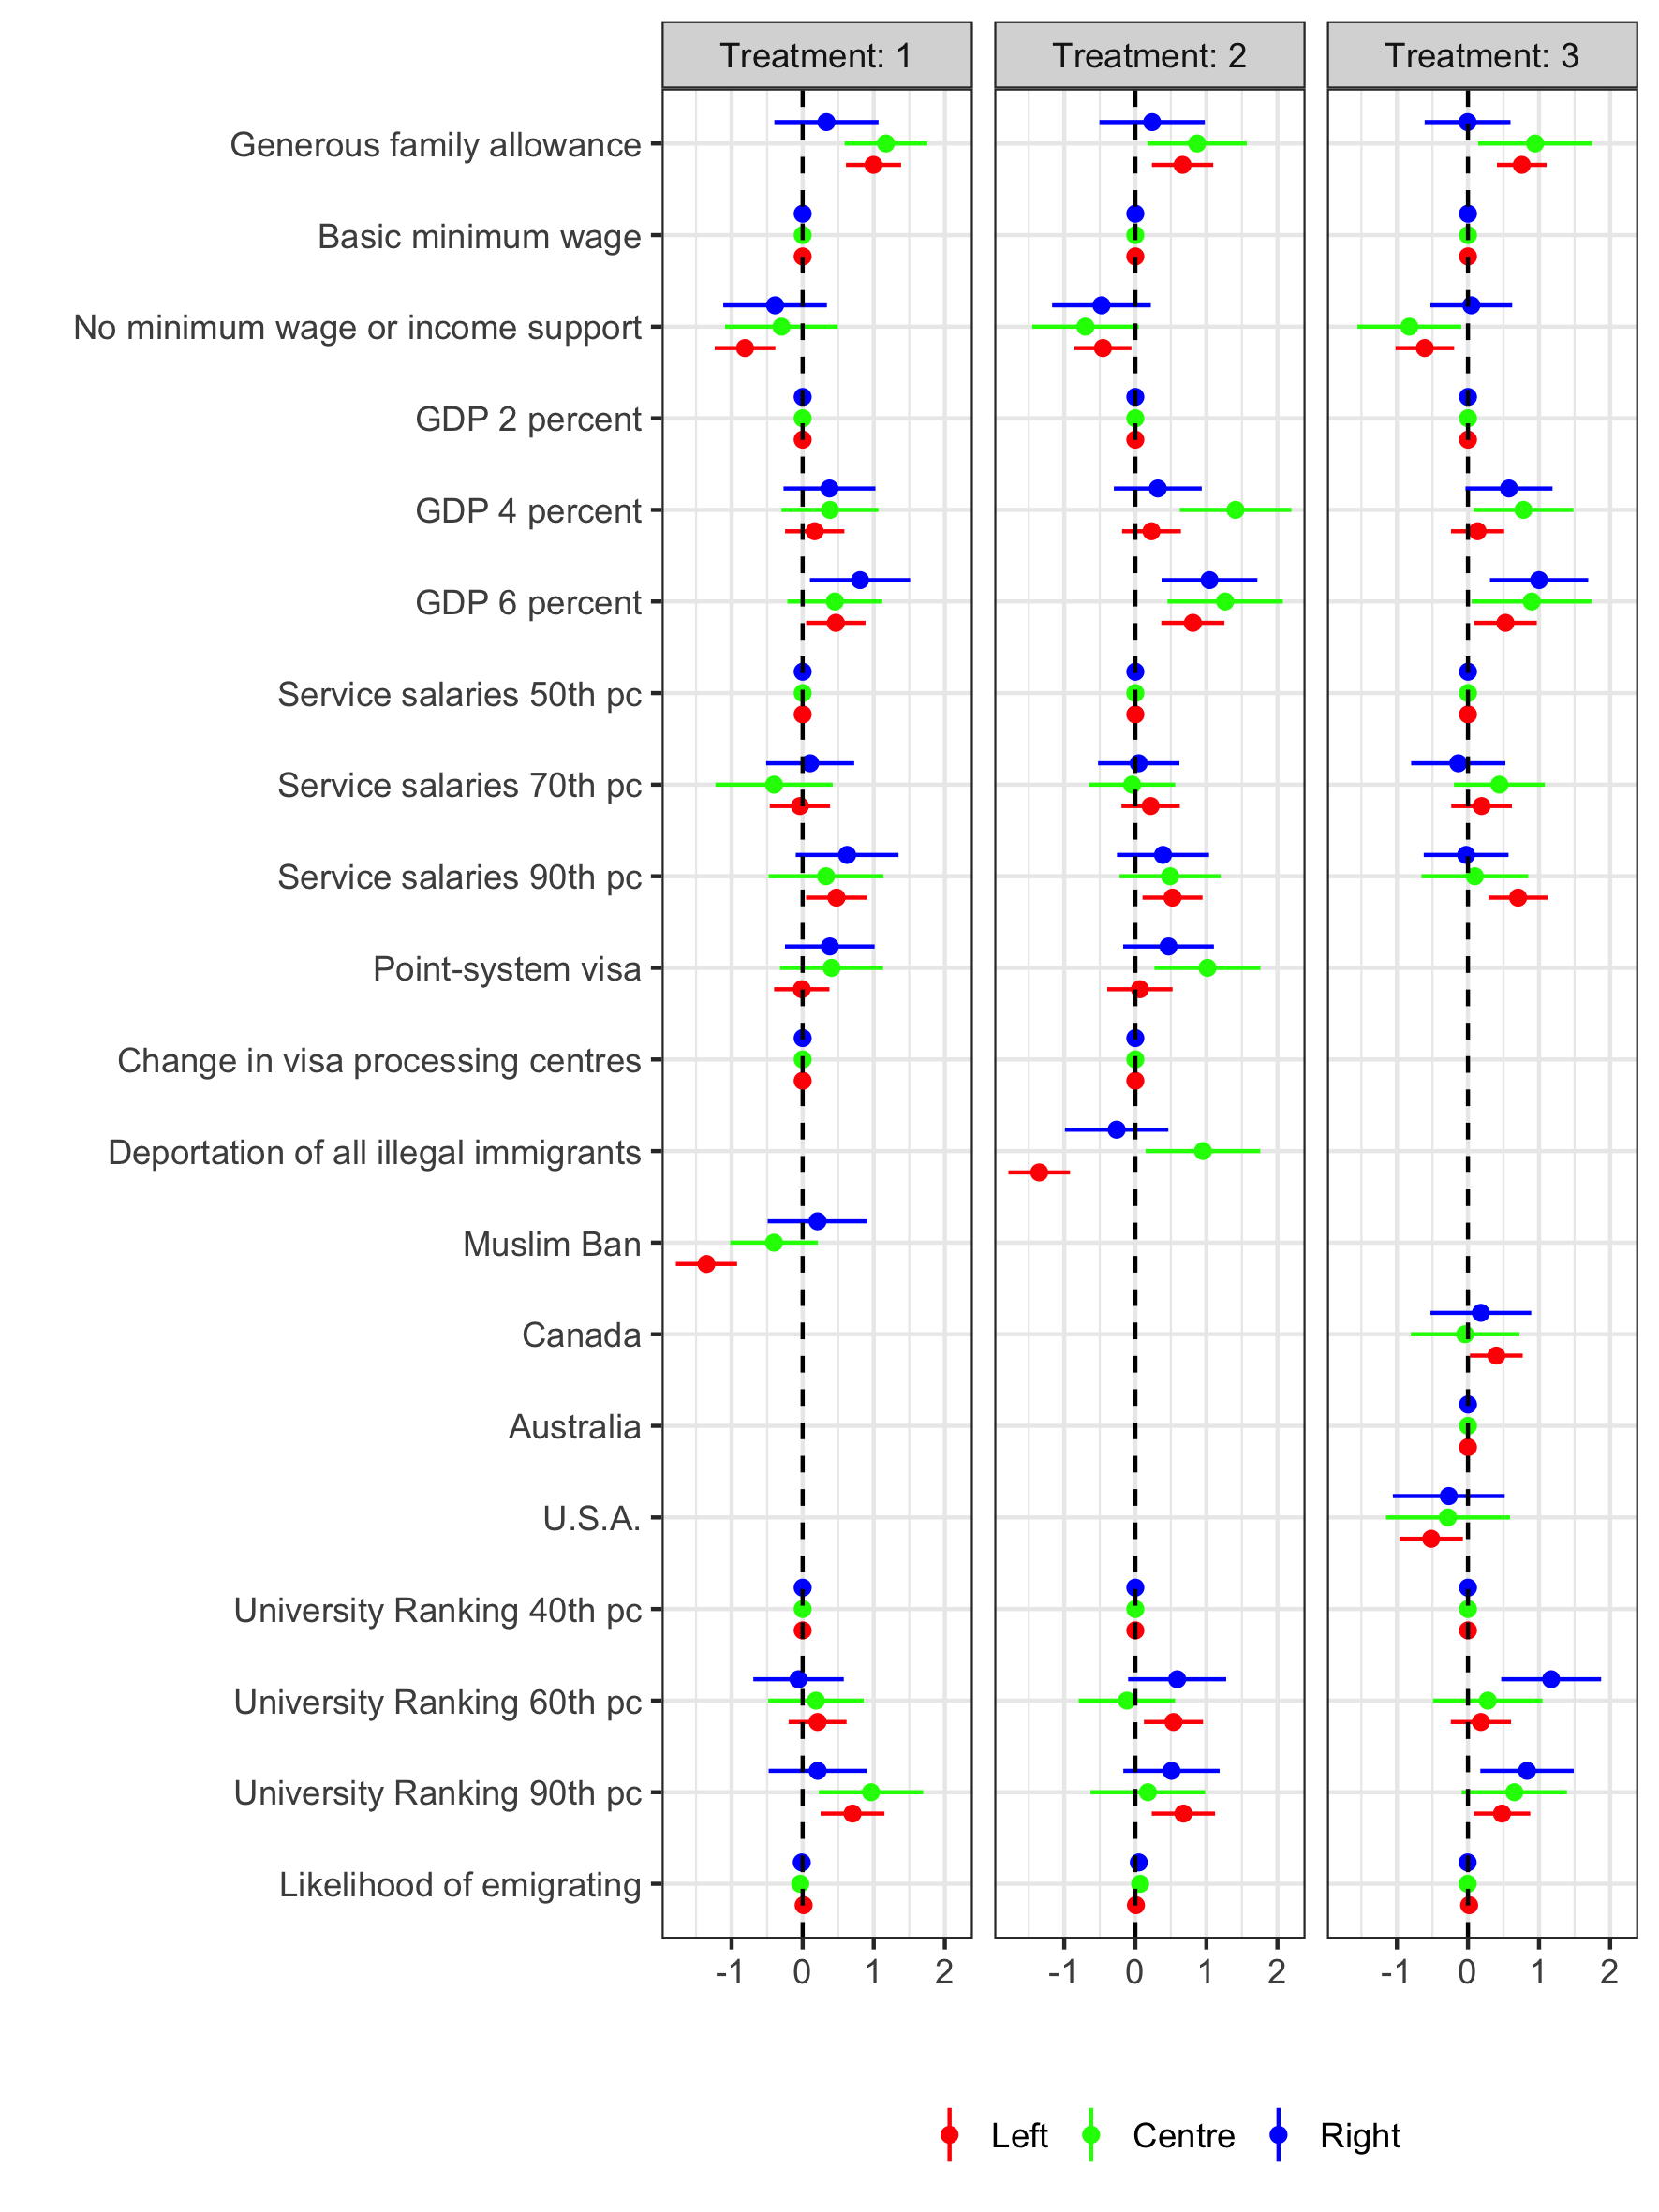
\includegraphics[scale=0.25]{conjoint_ideology.png}}
\end{figure}

\paragraph{Left-Right Divide.}  We conjectured above that potential emigrants may have partisan leanings that might affect their preferences for different employment destinations. Table~\ref{tab:subjects} (online appendix) suggests that the Oxford current and former student subject pool had a slightly disproportionately large number of subjects that identify as Left on the Left-Right self-placement scale. The tendency for subjects to self-place on the Left may partly explain the preferences for destination countries with generous welfare benefits as well as the antipathy for countries with anti-immigrant policies.

\par We divided the subjects into Left, Center, and Right groups and then estimated the same conjoint models that were presented in Figure~\ref{fig:treatment_combined}.\note{Participants on the Left were operationally defined as those who indicated they were 4 or lower on an 11-point scale, Center those who selected 5, and Right those who selected 6 or more.}  Figure~\ref{fig:conjoint_ideology} presents the graphical results from these three models.\note{The numeric logistic estimations are presented in Tables ~\ref{tab:results_breakout1}--\ref{tab:results_breakout3} in the online appendix.}  Clearly, politics matters!  Participants who self-identify as on the political right are almost exclusively concerned with economic performance in all three immigration treatments -- they favor employment destinations that have high GDP growth and high service sector salaries. In addition to these economic factors, Left-leaning subjects appear to be very much concerned about immigration policy and social welfare. They were clearly put-off by the immigration treatments that mentioned a ``Muslim Ban'' and ``Deportation of Illegal Immigrants,'' and they were deterred by the US as a migration destination. Finally, they responded positively to destinations with highly ranked universities, albeit less so than Right-leaning subjects.

%\clearpage


\section*{Conclusion and Discussion}

\par The UK has historically witnessed comparatively high levels of emigration to countries throughout the world (in particular to its former colonies).  And in a post-Brexit world some expect these numbers to rise.  Where will the British go?  Traditionally, the United States has been a favored destination for UK emigrants, particularly the highly skilled.  This essay examines whether the recent immigration politics and policies in the US have negatively affected its ability to attract high skilled immigrants. 

\par The findings from our conjoint experiment suggest that both the economy and politics matter for UK emigrants. Politics is of particular concern to potential emigrants on the Left and Center while economic considerations shape the destination preferences of all potential emigrants. 

\par In general, anti-immigrant rhetoric seems to discourage highly skilled potential emigrants from the UK. Moreover, the `Trumpian' policies and rhetoric seem to have tarnished the US brand, at least for the highly skilled participants in our sample. In line with our conjectures, the US is not currently viewed as favorably as Canada or Australia and associating the ``US'' with skilled job offers significantly reduces their appeal to prospective high-skilled employees. 

\par Furthermore, associating `Trumpian' immigration policy proposals, such as the ``Muslim Ban'' and ``Deportation of illegal migrants,'' with an employment destination strongly reduces its attractiveness to potential high-skilled immigrants. However these predispositions have a strong partisan flavor, with those on the political left less likely, than those on the right, to choose the US as an emigration destination and less likely to select one associated with `Trumpian' immigration policies.
%Migrations decisions of those on the Left and Center also appear to be driven by the availability of social benefits, preferring destinations with generous family allowances and rejecting those that do not have minimum wage or income support. 

\par Consistent with our conjectures, destinations with higher economic growth and better universities are more attractive -- though education is not a strong driver of these choices. These results suggest that countries like the US with high salaries and universities of excellence, are attractive destinations for high-skilled labor, especially for potential migrants on the political right. There are, on the other hand, aspects of the US economy and current immigration policies that will dissuade highly skilled immigrants from the UK: skilled migrants from the UK, on both the political left and right, prefer destinations with generous social benefits; and high-skilled migrants are dissuaded by populist or nativist politics.

\par Our effort to understand how US politics and economic fundamentals shape the migration decision of highly skilled immigrants is based on potential skilled migrants from the UK. Ongoing research will explore whether these migration preferences generalize to the broader global talent pool from which the USA attracts skilled immigration. 

%\par The findings of the conjoint treatments one and two, which do not include references to the USA, led us to believe that the potential negative effects of populist or nativist policies are independent of the country brand and could, therefore, affect any country where those political views are popular.


%on the other hand, both the Right and Left potential highly skilled emigrants from the UK are concerned about economic performance 



%We conclude.....
%\begin{itemize}
%\item we design a conjoint experiment to help us understand the political economy of migration by highly skilled individuals
%\item the economy matters for all potential emigrants -- successful national economies are critical for all potential emigrants
%\item politics also matters although as you would expect it depends on the partisan orientation of the potential emigrants.
%\item In general, immigration policies are a strong signal dissuading UK highly skilled emigrants -- and the policies adopted by Trump seem to have tarnished the US brand - at least for UK highly skilled emigrants
%\item but the UK highly skilled emigrants -- or at least the ones in our samples (the elite potential emigrants) -- have a strong partisan flavor -- not surprisingly maybe they are left-wing...
%\item the immigration policy concerns of potential highly skilled emigrants are concentrated amongst the Left -- the Right are indifferent
%\item similarly the Left is attracted by government largese... and the Right is also indifferent to social welfare infrastructure
%\item on the other hand, both the Right and Left potential highly skilled emigrants from the UK are concerned about economic performance 

%\end{itemize}


%\newpage
%\begin{singlespace}
\bibliography{dave}
%\end{singlespace}

\pagebreak


\begin{appendices}
\setcounter{section}{0}
\renewcommand\thesection{\Alph{section}}
\renewcommand\thesubsection{\Alph{section}\arabic{subsection}}
\renewcommand\thefigure{\Alph{section}\arabic{figure}}
\renewcommand\thetable{\Alph{section}\arabic{table}}

%\section{Experiment design.}
\setcounter{table}{0}
\setcounter{figure}{0}


\label{Appendix_Design}

\section{Screenshots}

\setcounter{page}{1}

\begin{figure}[H]
\caption{Screenshot conjoint treatment 1}\label{fig:screen_one}
\centerline{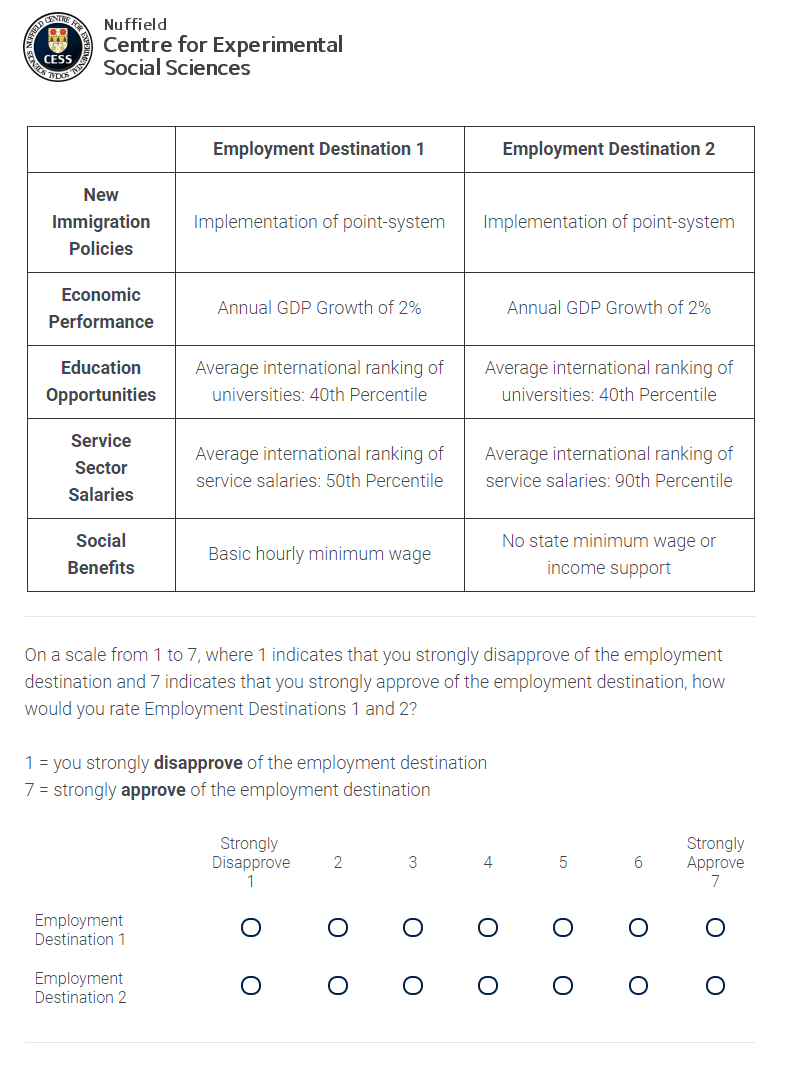
\includegraphics[width=\textwidth, height=0.85\textheight]{Screenshot_conjoint1}}
\end{figure}

\begin{figure}[H]
\caption{Screenshot conjoint treatment 2}\label{fig:screen_two}
\centerline{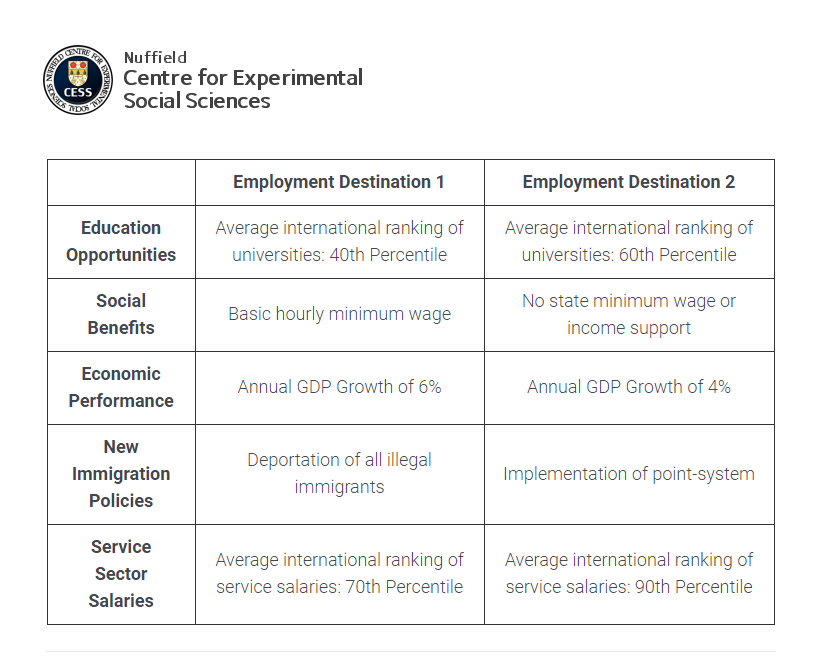
\includegraphics[width=\textwidth, height=0.6\textheight]{Screenshot_conjoint2}}
\end{figure}

\begin{figure}[H]
\caption{Screenshot conjoint treatment 3}\label{fig:screen_three}
\centerline{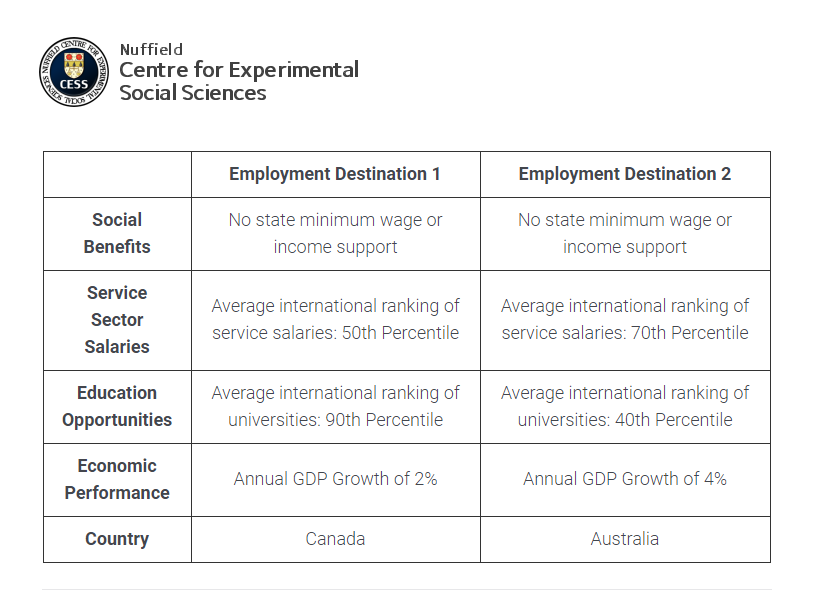
\includegraphics[width=\textwidth, height=0.6\textheight]{Screenshot_conjoint3}}
\end{figure}

\section{Descriptives}



%\clearpage

\singlespace



\par Table~\ref{tab:subjects} presents summary statistics for age, gender and ideological self-placement of the participants, as well their interest in emigrating, their likelihood of emigrating and how favorably they rate Australia, Canada, and the USA as employment destinations. As expected with a current and former student subject pool, participants are predominantly young, but there are a few older participants in the sample. Female participants (56 percent) slightly outnumber males. The ideological preferences of subjects has a fairly normal distribution although, as we expected with student subjects, these are skewed somewhat to the left. Density plots of age and ideological self-placement are below. Participants' interest in migration is relatively high, with a mean of 5.5 on a 1--7 point scale, indicating the relevance of the subject pool as representatives of potential high skilled migrants. The self-reported likelihood of emigrating is also high, with a mean of 4.9 on a 1--7 point scale, however, somewhat lower than interest in migration. Including a control for the likelihood of migration in the logit analysis does not alter the results of the estimation (see Table~\ref{tab:results_controls}).

\begin{table}[!htbp]
\caption{Characteristics of the Subject Pool and summary statistics}\label{tab:subjects}
\begin{center}
\begin{tabular}{llllll}
  \hline
\textbf{Variable} & \textbf{Mean} & \textbf{SD} & \textbf{Min}. & \textbf{Max}. & \textbf{N} \\ 
  \hline
Age & 25.81 & 8.6 & 19 & 68 & 196 \\
Female & 0.56 & 0.5 & 0 & 1 & 196 \\
Ideology & 4.1 & 1.84 & 0 & 10 & 196 \\
Interest in emigrating & 5.48 & 1.48 & 1 & 7 & 195 \\ 
Likelihood of emigrating & 4.91 & 1.76 & 1 & 7 & 195 \\
  \hline
Employment destination perceptions: & & & & & \\
   \hline
 Australia & 5.18 & 1.26 & 1 & 7 & 196 \\ 
  Canada & 5.6 & 1.27 & 1 & 7 & 196 \\ 
  U.S.A. & 4.61 & 1.65 & 1 & 7 & 196 \\ 
  \hline
  \textbf{Conjoint attribute variables} & & & & & \\
  \hline
  Basic hourly minimum wage & 0.32 & 0.46 & 0 & 1 & 1112 \\ 
  Generous guaranteed monthly  & &  & &  &  \\
  family allowance & 0.34 & 0.47 & 0 & 1 & 1212 \\ 
  No state minimum wage  & &  & &  &  \\
  or income support & 0.34 & 0.47 & 0 & 1 & 1204 \\ 
  Annual GDP Growth of 2\% & 0.34 & 0.47 & 0 & 1 & 1200 \\ 
  Annual GDP Growth of 4\% & 0.34 & 0.47 & 0 & 1 & 1191 \\ 
  Annual GDP Growth of 6\% & 0.32 & 0.47 & 0 & 1 & 1137 \\ 
  Service salaries: 50th Percentile & 0.35 & 0.48 & 0 & 1 & 1236 \\ 
  Service salaries: 70th Percentile & 0.33 & 0.47 & 0 & 1 & 1168 \\ 
  Service salaries: 90th Percentile & 0.32 & 0.47 & 0 & 1 & 1124 \\ 
  Change in visa processing centres & 0.22 & 0.41 & 0 & 1 & 776 \\ 
  Implementation of point-system & 0.22 & 0.41 & 0 & 1 & 770 \\ 
  Restriction on Muslim   & &  & &  &  \\
  immigration/tourist visas & 0.11 & 0.32 & 0 & 1 & 397 \\ 
  Deportation of all illegal immigrants & 0.12 & 0.32 & 0 & 1 & 409 \\ 
  Country label: Australia & 0.12 & 0.32 & 0 & 1 & 413 \\ 
  Country label: Canada & 0.11 & 0.31 & 0 & 1 & 392 \\ 
  Country label: U.S.A. & 0.11 & 0.31 & 0 & 1 & 371 \\ 
  Ranking of universities: 40th Percentile & 0.34 & 0.47 & 0 & 1 & 1195 \\ 
  Ranking of universities: 60th Percentile & 0.33 & 0.47 & 0 & 1 & 1164 \\ 
  Ranking of universities: 90th Percentile & 0.33 & 0.47 & 0 & 1 & 1169 \\ 
   \hline
\end{tabular}
\end{center}
\end{table}


The overall employment destination perceptions (middle section Table \ref{tab:subjects}) indicate that participants significantly favored Canada and Australia, relative to the US ($p<0.000$ and $p = 0.000137$ for pairwise comparisons). This is possibly associated with the slightly more female and left wing composition of the subject pool. However, the negative evaluation of the US brand is also present in the logit estimations in Table~\ref{tab:results} and is sustained when we incorporate controls for age and gender (Table~\ref{tab:results_controls}).

The bottom section of the table presents the proportion (exemplified by the mean) of the participants that observed each attribute in the conjoint experiments. Roughly $1/3$ of the participants saw each of the socio-economic alternatives. Since the immigration alternatives were varied across the three treatments, we expect to see the country label and negative treatment attributes roughly $1/9$ of the time. However, the neutral (`Change in visa processing centers') and positive alternatives (`Implementation of point-system') were held constant across immigration treatments one and two. These attributes should therefore have been presented twice as often ($2/9$). The proportions of observed attributes (Table~\ref{tab:subjects}) are in line with expectations of a successful randomization. Further balance tests on randomization of conjoint attributes (see online appendix) indicate that socio-demographic variables are not significant predictors of observing an attribute. One notable exception is the lower probability of observing Canada for those most interested in migrating. Given this significant association, we included migration interest as a control variable in the models. However, it is not a substantive or consistent predictor of destination choice and omitting it does not alter the results (data in replication material).\note{The `Other' gender category also appears significant in the balance tests, as merely one respondent selected this category. Age has a significant association with the likelihood of observing `No state minimum wage' relative to `Basic minimum wage'; however, it is not associated with any other of the conjoint attributes and including `Age' as a control does not alter the results of the estimations.}


\begin{figure}[!ht]
\caption{Age Distribution of UK Subject Pool}\label{fig:describe_one}
\centerline{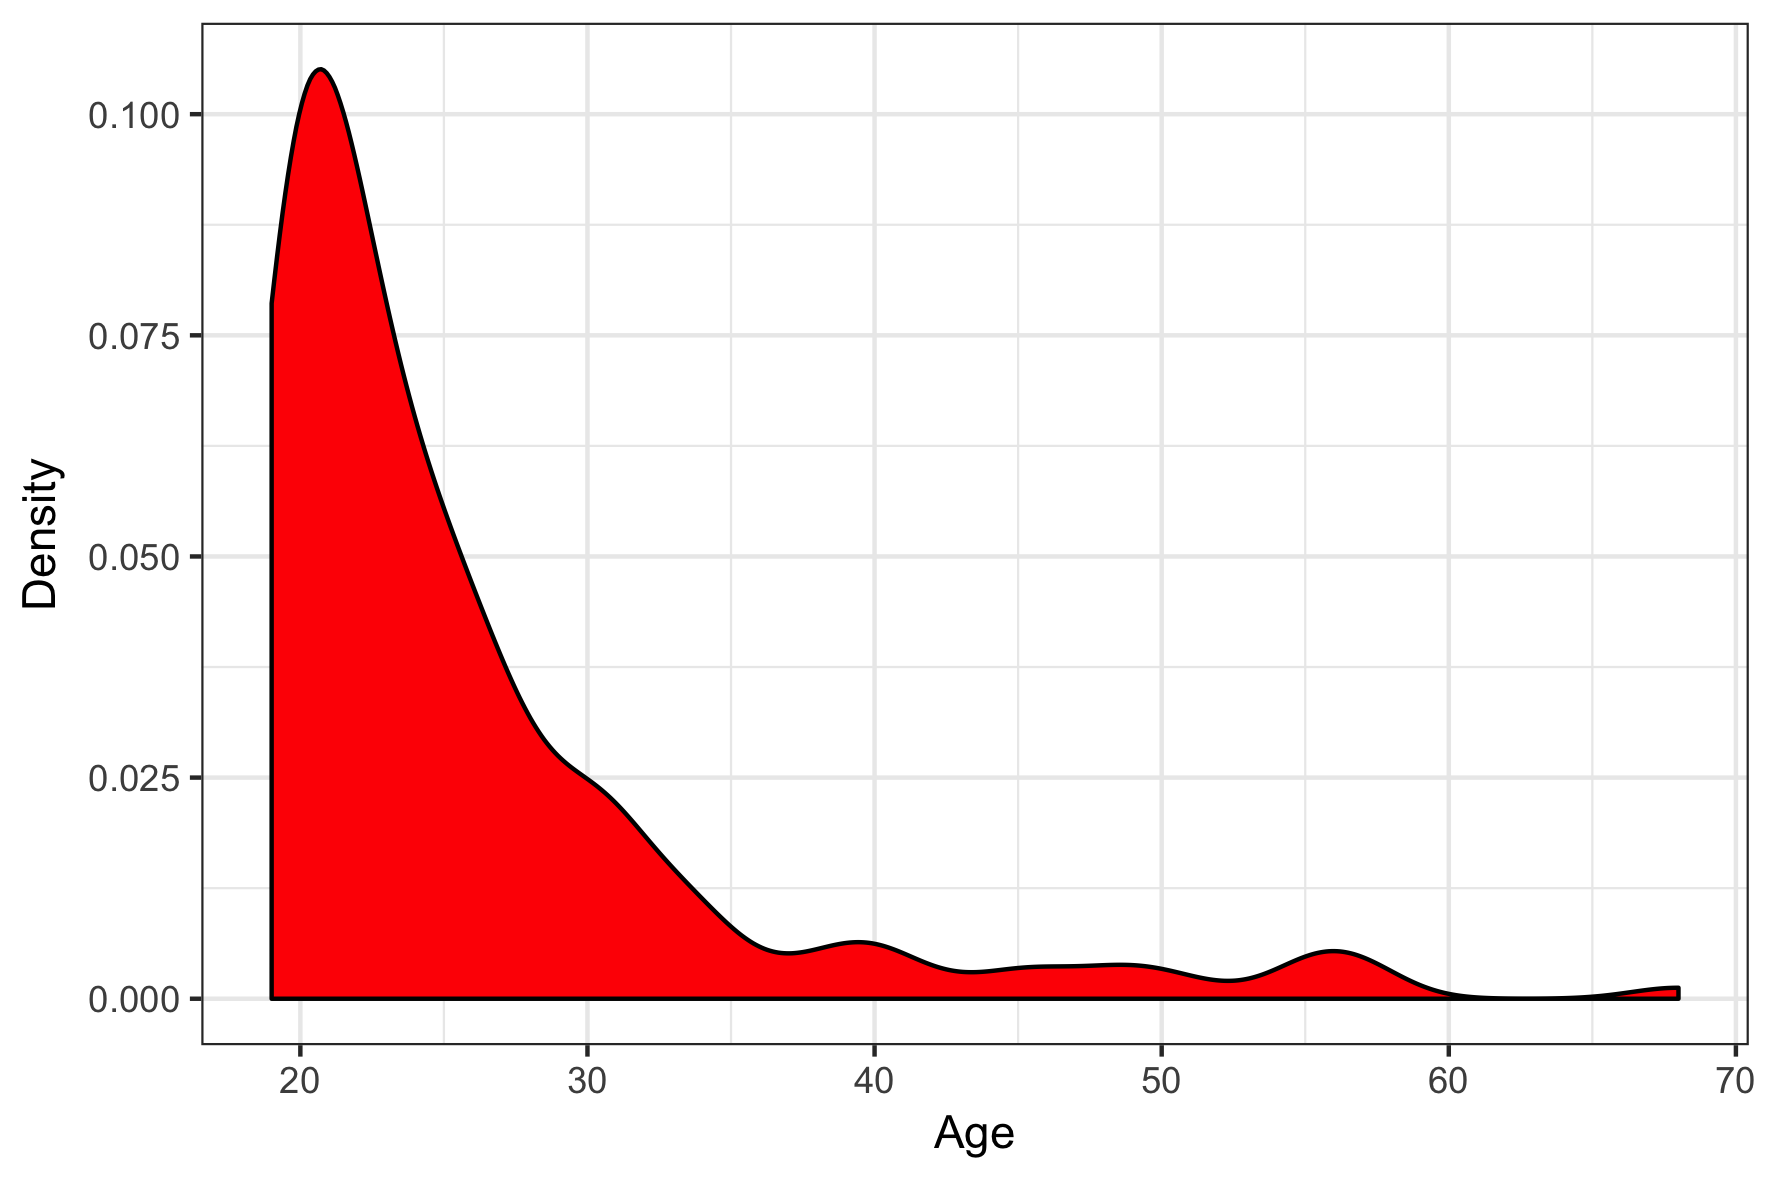
\includegraphics[scale=0.25]{age.png}}
\end{figure}

\clearpage

\begin{figure}[!ht]
\caption{Gender Distribution of UK Subject Pool}\label{fig:describe_two}
\centerline{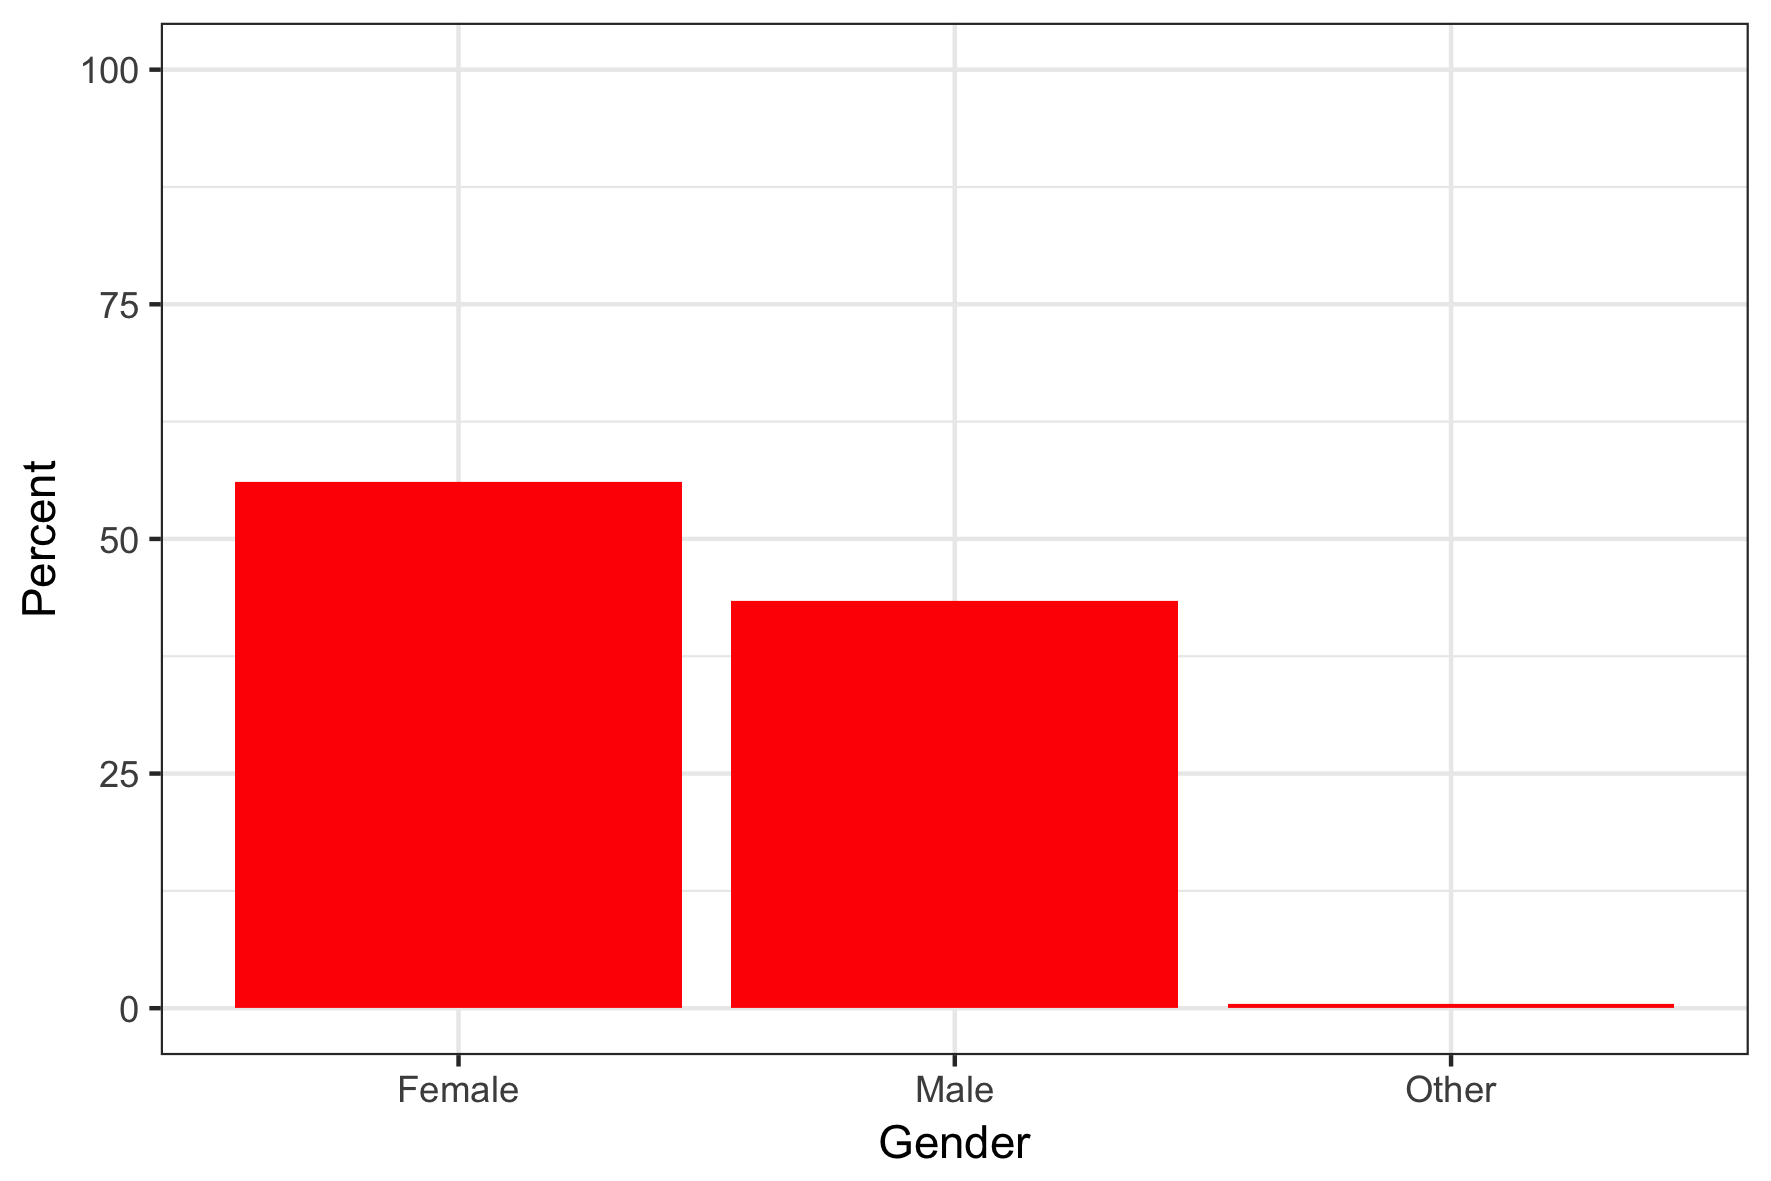
\includegraphics[scale=0.25]{gender.png}}
\end{figure}

\clearpage

\begin{figure}[!ht]
\caption{Ideological Distribution of UK Subject Pool}\label{fig:describe_three}
\centerline{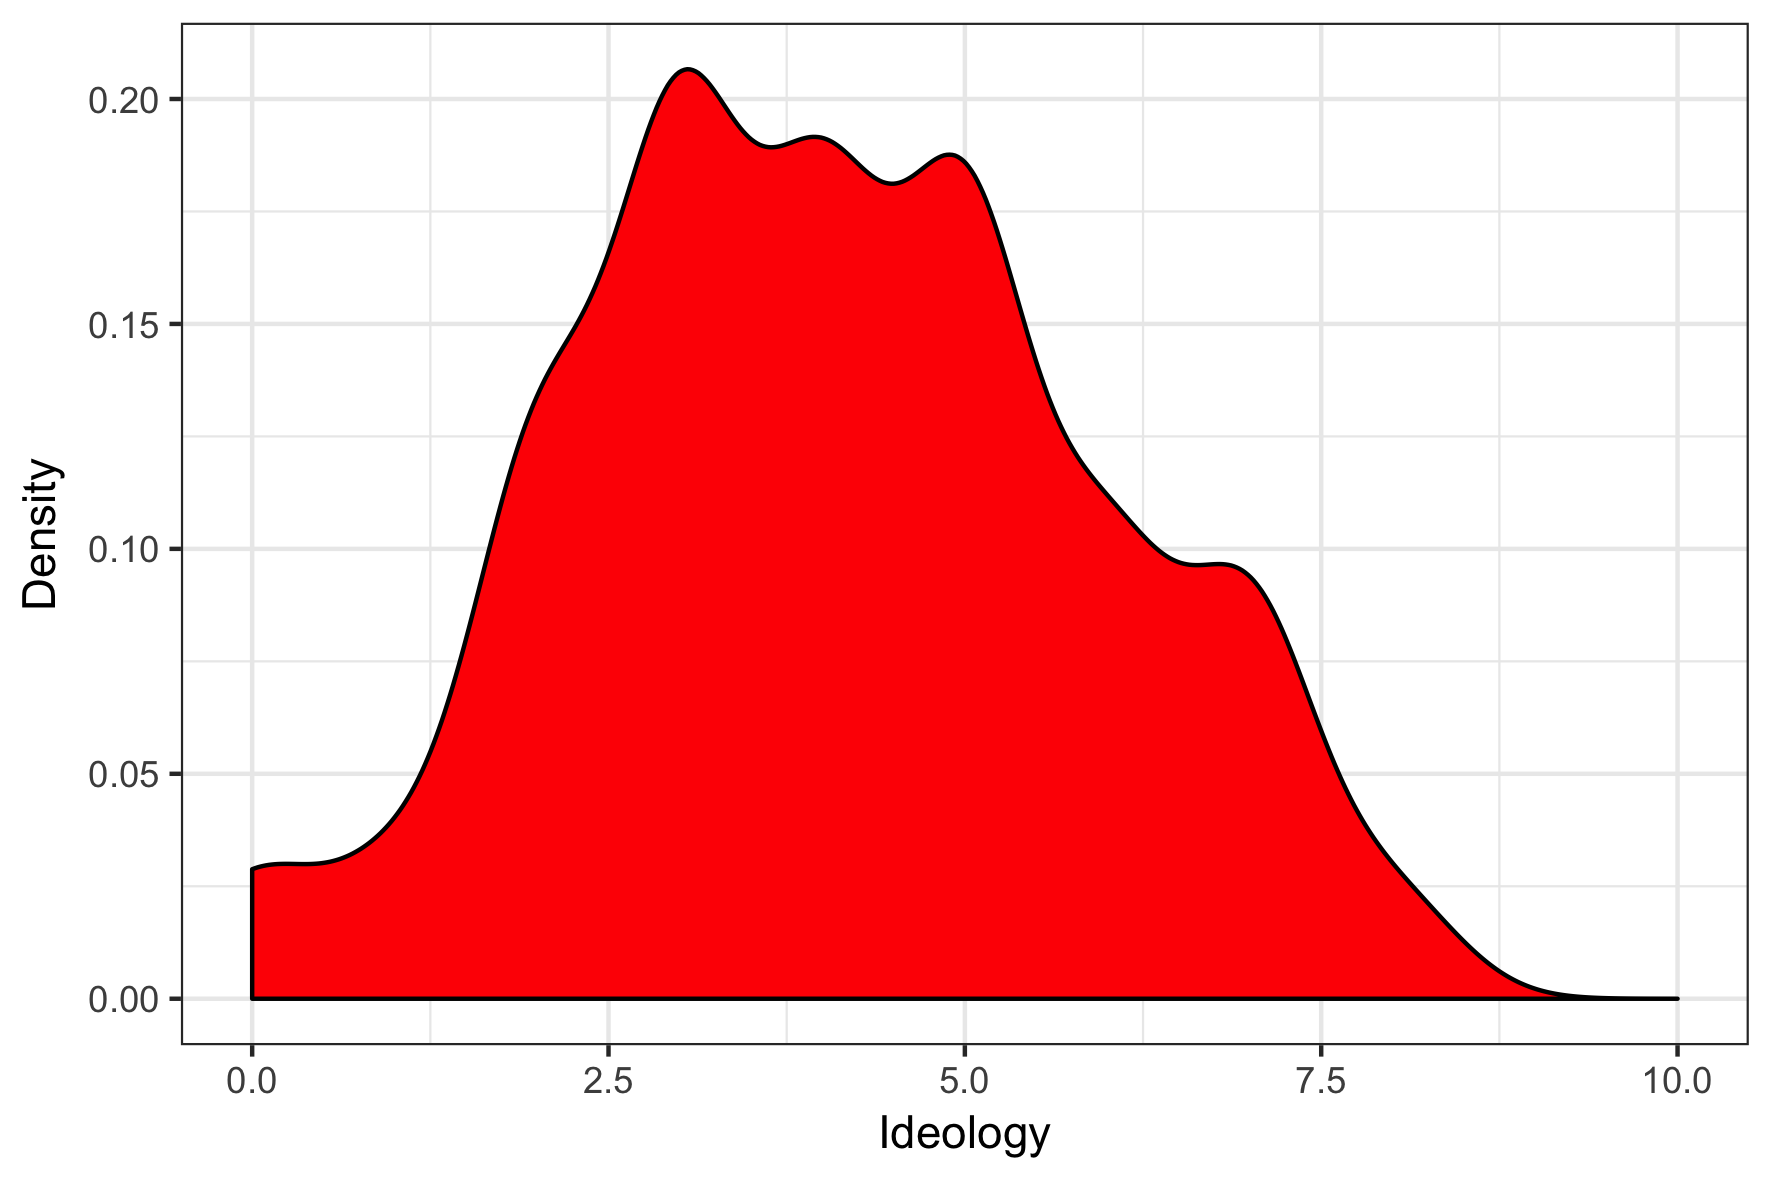
\includegraphics[scale=0.25]{ideology.png}}
\end{figure}


\section{Main model table}
\clearpage

\begin{table}[H] \centering 
  \caption{Logistic regression results} 
  \label{tab:results} 
\begin{tabular}{@{\extracolsep{5pt}}lccc} 
\\[-1.8ex]\hline 
\hline \\[-1.8ex] 
 & \multicolumn{3}{c}{Immigration Treatment} \\ 
\cline{2-4} 
\\[-1.8ex] & (1) & (2) & (3)\\ 
\hline \\[-1.8ex] 
 Generous family allowance & 0.765$^{***}$ & 0.557$^{***}$ & 0.555$^{***}$ \\ 
  & (0.151) & (0.159) & (0.138) \\ 
  No minimum wage or income support & $-$0.635$^{***}$ & $-$0.511$^{***}$ & $-$0.513$^{***}$ \\ 
  & (0.168) & (0.157) & (0.154) \\ 
  GDP 2 percent & $-$0.253 & $-$0.381$^{**}$ & $-$0.307$^{**}$ \\ 
  & (0.155) & (0.153) & (0.150) \\ 
  GDP 6 percent & 0.304$^{**}$ & 0.473$^{***}$ & 0.366$^{**}$ \\ 
  & (0.155) & (0.157) & (0.146) \\ 
  Service salaries 50th pc & 0.098 & $-$0.134 & $-$0.168 \\ 
  & (0.160) & (0.148) & (0.159) \\ 
  Service salaries 90th pc & 0.530$^{***}$ & 0.343$^{**}$ & 0.233 \\ 
  & (0.159) & (0.152) & (0.149) \\ 
  Deportation of all illegal immigrants &  & $-$0.662$^{***}$ &  \\ 
  &  & (0.176) &  \\ 
  Point-system visa & 0.125 & 0.342$^{**}$ &  \\ 
  & (0.151) & (0.170) &  \\ 
  Muslim Ban & $-$0.787$^{***}$ &  &  \\ 
  & (0.162) &  &  \\ 
  Canada &  &  & 0.272$^{*}$ \\ 
  &  &  & (0.150) \\ 
  U.S.A. &  &  & $-$0.345$^{**}$ \\ 
  &  &  & (0.174) \\ 
  University Ranking 40th pc & $-$0.139 & $-$0.417$^{***}$ & $-$0.384$^{**}$ \\ 
  & (0.150) & (0.154) & (0.164) \\ 
  University Ranking 90th pc & 0.476$^{***}$ & 0.122 & 0.183 \\ 
  & (0.151) & (0.157) & (0.158) \\ 
  Likelihood of emigrating & $-$0.012 & 0.023$^{*}$ & 0.014 \\ 
  & (0.014) & (0.014) & (0.011) \\ 
  Constant & $-$0.092 & 0.003 & $-$0.019 \\ 
  & (0.213) & (0.199) & (0.201) \\ 
 \hline \\[-1.8ex] 
Observations & 1,170 & 1,170 & 1,170 \\ 
Log Likelihood & $-$731.956 & $-$740.916 & $-$759.410 \\ 
Akaike Inf. Crit. & 1,487.913 & 1,505.832 & 1,542.820 \\   
\hline 
\hline \\[-1.8ex] 
\multicolumn{4}{l}{ \textit{Note:} $^{*}$p$<$0.1; $^{**}$p$<$0.05; $^{***}$p$<$0.01 }  \\ 
\multicolumn{4}{l}{\textit{Standard errors clustered by participant}}
\end{tabular} 
\end{table} 
%\clearpage

\section{Additional models}
%Model with controls - updated to include likelihood
%\clearpage

\begin{table}[H] \centering \small
  \caption{Logistic regression results including control variables} 
  \label{tab:results_controls}
\begin{tabular}{@{\extracolsep{5pt}}lccc} 
\\[-1.8ex]\hline 
\hline \\[-1.8ex] 
 & \multicolumn{3}{c}{Immigration Treatment} \\ 
\cline{2-4} 
\\[-1.8ex] & (1) & (2) & (3)\\ 
\hline \\[-1.8ex] 
Generous family allowance & 0.769$^{***}$ & 0.556$^{***}$ & 0.557$^{***}$ \\ 
  & (0.153) & (0.160) & (0.138) \\ 
  No minimum wage or income support & $-$0.637$^{***}$ & $-$0.514$^{***}$ & $-$0.527$^{***}$ \\ 
  & (0.169) & (0.158) & (0.155) \\ 
  GDP 2 percent & $-$0.252 & $-$0.383$^{**}$ & $-$0.303$^{**}$ \\ 
  & (0.155) & (0.153) & (0.150) \\ 
  GDP 6 percent & 0.307$^{**}$ & 0.478$^{***}$ & 0.370$^{**}$ \\ 
  & (0.156) & (0.158) & (0.146) \\ 
  Service salaries 50th pc & 0.102 & $-$0.136 & $-$0.174 \\ 
  & (0.161) & (0.148) & (0.160) \\ 
  Service salaries 90th pc & 0.528$^{***}$ & 0.339$^{**}$ & 0.235 \\ 
  & (0.159) & (0.152) & (0.150) \\ 
  Deportation of all illegal immigrants &  & $-$0.662$^{***}$ &  \\ 
  &  & (0.176) &  \\ 
  Point-system visa & 0.131 & 0.346$^{**}$ &  \\ 
  & (0.152) & (0.170) &  \\ 
  Muslim Ban & $-$0.790$^{***}$ &  &  \\ 
  & (0.162) &  &  \\ 
  Canada &  &  & 0.281$^{*}$ \\ 
  &  &  & (0.150) \\ 
  U.S.A. &  &  & $-$0.346$^{**}$ \\ 
  &  &  & (0.175) \\ 
  University Ranking 40th pc & $-$0.141 & $-$0.418$^{***}$ & $-$0.389$^{**}$ \\ 
  & (0.150) & (0.155) & (0.165) \\ 
  University Ranking 90th pc & 0.482$^{***}$ & 0.126 & 0.175 \\ 
  & (0.152) & (0.158) & (0.158) \\ 
  Age & $-$0.006$^{**}$ & $-$0.001 & $-$0.003 \\ 
  & (0.002) & (0.002) & (0.002) \\ 
  Gender: Male & 0.020 & $-$0.025 & $-$0.013 \\ 
  & (0.047) & (0.046) & (0.040) \\ 
  Gender: Other & $-$0.196 & 0.346$^{***}$ & 0.735$^{***}$ \\ 
  & (0.127) & (0.094) & (0.145) \\ 
  Ideological self-placement & $-$0.005 & $-$0.013 & $-$0.001 \\ 
  & (0.013) & (0.012) & (0.010) \\ 
  Likelihood of emigrating & $-$0.012 & 0.023$^{*}$ & 0.015 \\ 
  & (0.014) & (0.014) & (0.011) \\ 
  Constant & 0.077 & 0.100 & 0.071 \\ 
  & (0.231) & (0.219) & (0.208) \\ 
 \hline \\[-1.8ex] 
Observations & 1,170 & 1,170 & 1,170 \\ 
Log Likelihood & $-$731.562 & $-$740.666 & $-$758.904 \\ 
Akaike Inf. Crit. & 1,495.124 & 1,513.333 & 1,549.808 \\    
\hline 
\hline \\[-1.8ex] 
\textit{Note:}  & \multicolumn{3}{r}{$^{*}$p$<$0.1; $^{**}$p$<$0.05; $^{***}$p$<$0.01} \\
\multicolumn{4}{r}{\textit{Standard errors clustered by participant}}
\end{tabular} 
\end{table}


%Check where conjoint presents same country in both employment destinations

\begin{table}[!htbp] \centering 
  \caption{Comparison of logistic results for treatment 3 by country pair} 
  \label{tab:results_samecountry}
\begin{tabular}{@{\extracolsep{5pt}}lcc} 
\\[-1.8ex]\hline 
\hline \\[-1.8ex] 
 & \multicolumn{2}{c}{Country Pair} \\ 
\cline{2-3} 
\\[-1.8ex] & Non-identical & Identical\\ 
\hline \\[-1.8ex] 
  Generous family allowance & 0.338$^{*}$ & 0.961$^{***}$ \\ 
  & (0.177) & (0.267) \\ 
  No minimum wage or income support & $-$0.409$^{**}$ & $-$0.755$^{***}$ \\ 
  & (0.193) & (0.264) \\ 
  GDP 2 percent & $-$0.248 & $-$0.235 \\ 
  & (0.176) & (0.279) \\ 
  GDP 6 percent & 0.433$^{**}$ & 0.448 \\ 
  & (0.172) & (0.280) \\ 
  Service salaries 50th pc & $-$0.112 & $-$0.278 \\ 
  & (0.184) & (0.281) \\ 
  Service salaries 90th pc & 0.258 & 0.208 \\ 
  & (0.180) & (0.277) \\ 
  Canada & 0.381$^{*}$ & 0.142 \\ 
  & (0.225) & (0.111) \\ 
  U.S.A. & $-$0.508$^{**}$ & 0.001 \\ 
  & (0.245) & (0.119) \\ 
  University Ranking 40th pc & $-$0.531$^{***}$ & $-$0.184 \\ 
  & (0.204) & (0.272) \\ 
  University Ranking 90th pc & $-$0.065 & 0.648$^{**}$ \\ 
  & (0.194) & (0.270) \\ 
  Age & $-$0.003 & $-$0.002 \\ 
  & (0.003) & (0.005) \\ 
  Gender: Male & 0.012 & $-$0.058 \\ 
  & (0.045) & (0.102) \\ 
  Gender: Other & 0.495$^{***}$ & 1.036$^{***}$ \\ 
  & (0.162) & (0.310) \\ 
  Ideological self-placement & $-$0.004 & $-$0.014 \\ 
  & (0.012) & (0.024) \\ 
  Likelihood of emigrating & 0.010 & $-$0.002 \\ 
  & (0.014) & (0.024) \\ 
  Constant & 0.211 & $-$0.171 \\ 
  & (0.271) & (0.365) \\ 
 \hline \\[-1.8ex] 
Observations & 772 & 398 \\ 
Log Likelihood & $-$503.758 & $-$244.928 \\ 
Akaike Inf. Crit. & 1,039.515 & 521.855 \\ 
\hline 
\hline \\[-1.8ex] 
\textit{Note:}  & \multicolumn{2}{r}{$^{*}$p$<$0.1; $^{**}$p$<$0.05; $^{***}$p$<$0.01} \\ 
\multicolumn{3}{r}{\textit{Standard errors clustered by participant}}
\end{tabular} 
\end{table} 

%Group breakouts
\begin{landscape}
\begin{table}[!htbp] \centering \footnotesize
  \caption{Model breakouts by gender and ideology (Treatment 1)} 
  \label{tab:results_breakout1} 
\begin{tabular}{@{\extracolsep{5pt}}lccccc} 
\\[-1.8ex]\hline 
\hline \\[-1.8ex] 
 & \multicolumn{5}{c}{Breakout} \\
 \cline{2-6} \\
 & \multicolumn{2}{c}{\textbf{Gender}} & \multicolumn{3}{c}{\textbf{Ideology}} \\  
\cline{2-6} 
\\[-1.8ex] & \textit{Male} & \textit{Female} & \textit{Left} & \textit{Centre} & \textit{Right}\\ 
\hline \\[-1.8ex] 
 Generous family allowance & 0.949$^{***}$ & 0.622$^{***}$ & 0.997$^{***}$ & 1.172$^{***}$ & 0.335 \\ 
  & (0.233) & (0.213) & (0.198) & (0.297) & (0.374) \\ 
  No minimum wage or income support & $-$0.451$^{*}$ & $-$0.834$^{***}$ & $-$0.811$^{***}$ & $-$0.298 & $-$0.388 \\ 
  & (0.272) & (0.209) & (0.218) & (0.405) & (0.372) \\ 
  GDP 4 percent & 0.380$^{*}$ & 0.160 & 0.170 & 0.384 & 0.377 \\ 
  & (0.225) & (0.220) & (0.213) & (0.348) & (0.330) \\ 
  GDP 6 percent & 0.743$^{***}$ & 0.428$^{**}$ & 0.467$^{**}$ & 0.453 & 0.807$^{**}$ \\ 
  & (0.251) & (0.203) & (0.213) & (0.341) & (0.360) \\ 
  Service salaries 70th pc & $-$0.119 & $-$0.113 & $-$0.039 & $-$0.403 & 0.106 \\ 
  & (0.238) & (0.221) & (0.217) & (0.421) & (0.316) \\ 
  Service salaries 90th pc & 0.551$^{**}$ & 0.400$^{*}$ & 0.476$^{**}$ & 0.329 & 0.626$^{*}$ \\ 
  & (0.246) & (0.222) & (0.219) & (0.412) & (0.369) \\ 
  Point-system visa & 0.220 & 0.102 & $-$0.013 & 0.407 & 0.382 \\ 
  & (0.196) & (0.223) & (0.199) & (0.370) & (0.322) \\ 
  Muslim Ban & $-$0.186 & $-$1.260$^{***}$ & $-$1.353$^{***}$ & $-$0.403 & 0.209 \\ 
  & (0.238) & (0.219) & (0.220) & (0.315) & (0.358) \\ 
  University Ranking 60th pc & 0.221 & 0.092 & 0.210 & 0.187 & $-$0.058 \\ 
  & (0.238) & (0.199) & (0.208) & (0.343) & (0.325) \\ 
  University Ranking 90th pc & 0.685$^{***}$ & 0.593$^{***}$ & 0.702$^{***}$ & 0.962$^{**}$ & 0.211 \\ 
  & (0.252) & (0.228) & (0.229) & (0.374) & (0.352) \\ 
  Likelihood of emigrating & $-$0.008 & $-$0.012 & 0.014 & $-$0.034 & $-$0.013 \\ 
  & (0.019) & (0.022) & (0.022) & (0.042) & (0.024) \\ 
  Constant & $-$0.925$^{***}$ & $-$0.008 & $-$0.303 & $-$0.790$^{*}$ & $-$0.781 \\ 
  & (0.327) & (0.295) & (0.284) & (0.419) & (0.512) \\ 
 \hline \\[-1.8ex] 
Observations & 510 & 654 & 684 & 222 & 264 \\ 
Log Likelihood & $-$320.449 & $-$397.813 & $-$402.620 & $-$137.496 & $-$174.728 \\ 
Akaike Inf. Crit. & 664.898 & 819.627 & 829.239 & 298.992 & 373.455 \\ 
\hline 
\hline \\[-1.8ex] 
\textit{Note:}  & \multicolumn{5}{r}{Standard errors clustered by participant; $^{*}$p$<$0.1; $^{**}$p$<$0.05; $^{***}$p$<$0.01} \\ 
\end{tabular} 
\end{table} 
\end{landscape}

\clearpage

\begin{landscape}
\begin{table}[!htbp] \centering \footnotesize
  \caption{Model breakouts by gender and ideology (Treatment 2)} 
  \label{tab:results_breakout2} 
\begin{tabular}{@{\extracolsep{5pt}}lccccc} 
\\[-1.8ex]\hline 
\hline \\[-1.8ex] 
 & \multicolumn{5}{c}{Breakout} \\
 \cline{2-6} \\
 & \multicolumn{2}{c}{\textbf{Gender}} & \multicolumn{3}{c}{\textbf{Ideology}} \\  
\cline{2-6} 
\\[-1.8ex] & \textit{Male} & \textit{Female} & \textit{Left} & \textit{Centre} & \textit{Right}\\ 
\hline \\[-1.8ex] 
  Generous family allowance & 0.307 & 0.713$^{***}$ & 0.665$^{***}$ & 0.869$^{**}$ & 0.237 \\ 
  & (0.247) & (0.214) & (0.220) & (0.357) & (0.378) \\ 
  No minimum wage or income support & $-$0.676$^{***}$ & $-$0.437$^{**}$ & $-$0.456$^{**}$ & $-$0.702$^{*}$ & $-$0.476 \\ 
  & (0.249) & (0.202) & (0.205) & (0.382) & (0.354) \\ 
  GDP 4 percent & 0.307 & 0.419$^{**}$ & 0.228 & 1.410$^{***}$ & 0.316 \\ 
  & (0.222) & (0.212) & (0.211) & (0.401) & (0.315) \\ 
  GDP 6 percent & 0.842$^{***}$ & 0.808$^{***}$ & 0.810$^{***}$ & 1.264$^{***}$ & 1.044$^{***}$ \\ 
  & (0.257) & (0.223) & (0.227) & (0.414) & (0.344) \\ 
  Service salaries 70th pc & $-$0.027 & 0.279 & 0.215 & $-$0.045 & 0.048 \\ 
  & (0.213) & (0.206) & (0.209) & (0.309) & (0.292) \\ 
  Service salaries 90th pc & 0.352 & 0.569$^{***}$ & 0.523$^{**}$ & 0.489 & 0.389 \\ 
  & (0.249) & (0.217) & (0.216) & (0.364) & (0.330) \\ 
  Point-system visa & 0.868$^{***}$ & $-$0.033 & 0.065 & 1.015$^{***}$ & 0.468 \\ 
  & (0.254) & (0.225) & (0.234) & (0.380) & (0.326) \\
  Deportation of all illegal immigrants & $-$0.335 & $-$0.883$^{***}$ & $-$1.352$^{***}$ & 0.951$^{**}$ & $-$0.263 \\ 
  & (0.253) & (0.246) & (0.221) & (0.412) & (0.371) \\ 
  University Ranking 60th pc & 0.369 & 0.388$^{*}$ & 0.537$^{**}$ & $-$0.119 & 0.589$^{*}$ \\ 
  & (0.239) & (0.204) & (0.212) & (0.346) & (0.352) \\ 
  University Ranking 90th pc & 0.488$^{**}$ & 0.510$^{**}$ & 0.677$^{***}$ & 0.177 & 0.509 \\ 
  & (0.249) & (0.224) & (0.227) & (0.412) & (0.346) \\ 
  Likelihood of emigrating & 0.030 & 0.022 & 0.009 & 0.068$^{*}$ & 0.049$^{*}$ \\ 
  & (0.020) & (0.020) & (0.023) & (0.041) & (0.026) \\ 
  Constant & $-$0.966$^{***}$ & $-$0.850$^{***}$ & $-$0.633$^{**}$ & $-$2.054$^{***}$ & $-$1.232$^{**}$ \\ 
  & (0.370) & (0.328) & (0.311) & (0.617) & (0.577) \\ 
 \hline \\[-1.8ex] 
Observations & 510 & 654 & 684 & 222 & 264 \\ 
Log Likelihood & $-$320.405 & $-$411.187 & $-$414.744 & $-$132.023 & $-$170.605 \\ 
Akaike Inf. Crit. & 664.811 & 846.373 & 853.488 & 288.046 & 365.209 \\ 
\hline 
\hline \\[-1.8ex] 
\textit{Note:}  & \multicolumn{5}{r}{Standard errors clustered by participant; $^{*}$p$<$0.1; $^{**}$p$<$0.05; $^{***}$p$<$0.01} \\ 
\end{tabular} 
\end{table} 
\end{landscape}

\clearpage

\begin{landscape}
\begin{table}[!htbp] \centering \footnotesize
  \caption{Model breakouts by gender and ideology (Treatment 3)} 
  \label{tab:results_breakout3} 
\begin{tabular}{@{\extracolsep{5pt}}lccccc} 
\\[-1.8ex]\hline 
\hline \\[-1.8ex] 
 & \multicolumn{5}{c}{Breakout} \\
 \cline{2-6} \\
 & \multicolumn{2}{c}{\textbf{Gender}} & \multicolumn{3}{c}{\textbf{Ideology}} \\  
\cline{2-6} 
\\[-1.8ex] & \textit{Male} & \textit{Female} & \textit{Left} & \textit{Centre} & \textit{Right}\\ 
\hline \\[-1.8ex] 
 Generous family allowance & 0.627$^{***}$ & 0.485$^{**}$ & 0.757$^{***}$ & 0.945$^{**}$ & $-$0.006 \\ 
  & (0.182) & (0.212) & (0.178) & (0.409) & (0.308) \\ 
  No minimum wage or income support & $-$0.126 & $-$0.882$^{***}$ & $-$0.607$^{***}$ & $-$0.825$^{**}$ & 0.047 \\ 
  & (0.218) & (0.216) & (0.211) & (0.373) & (0.293) \\ 
  GDP 4 percent & 0.222 & 0.368$^{*}$ & 0.135 & 0.780$^{**}$ & 0.577$^{*}$ \\ 
  & (0.236) & (0.191) & (0.191) & (0.359) & (0.312) \\ 
  GDP 6 percent & 0.823$^{***}$ & 0.555$^{**}$ & 0.528$^{**}$ & 0.897$^{**}$ & 1.001$^{***}$ \\ 
  & (0.260) & (0.225) & (0.225) & (0.431) & (0.353) \\ 
  Service salaries 70th pc & 0.355 & 0.086 & 0.192 & 0.443 & $-$0.137 \\ 
  & (0.241) & (0.219) & (0.218) & (0.326) & (0.338) \\ 
  Service salaries 90th pc & 0.487$^{**}$ & 0.365$^{*}$ & 0.705$^{***}$ & 0.096 & $-$0.026 \\ 
  & (0.234) & (0.215) & (0.212) & (0.383) & (0.304) \\ 
  Canada & $-$0.002 & 0.524$^{***}$ & 0.399$^{**}$ & $-$0.040 & 0.182 \\ 
  & (0.239) & (0.194) & (0.189) & (0.390) & (0.362) \\ 
  U.S.A. & $-$0.280 & $-$0.393 & $-$0.518$^{**}$ & $-$0.282 & $-$0.270 \\ 
  & (0.252) & (0.243) & (0.228) & (0.445) & (0.402) \\ 
  University Ranking 60th pc & 0.495$^{**}$ & 0.261 & 0.182 & 0.278 & 1.171$^{***}$ \\ 
  & (0.251) & (0.217) & (0.216) & (0.393) & (0.359) \\ 
  University Ranking 90th pc & 0.549$^{**}$ & 0.583$^{***}$ & 0.478$^{**}$ & 0.653$^{*}$ & 0.831$^{**}$ \\ 
  & (0.255) & (0.196) & (0.204) & (0.378) & (0.335) \\ 
  Likelihood of emigrating & 0.012 & 0.005 & 0.016 & $-$0.004 & $-$0.005 \\ 
  & (0.017) & (0.018) & (0.019) & (0.036) & (0.032) \\ 
  Constant & $-$1.090$^{***}$ & $-$0.664$^{**}$ & $-$0.821$^{***}$ & $-$0.958$^{*}$ & $-$1.102$^{**}$ \\ 
  & (0.327) & (0.287) & (0.305) & (0.523) & (0.507) \\ 
 \hline \\[-1.8ex] 
Observations & 510 & 654 & 684 & 222 & 264 \\ 
Log Likelihood & $-$335.061 & $-$412.989 & $-$429.735 & $-$137.432 & $-$170.784 \\ 
Akaike Inf. Crit. & 694.123 & 849.978 & 883.470 & 298.864 & 365.567 \\ 
\hline 
\hline \\[-1.8ex] 
\textit{Note:}  & \multicolumn{5}{r}{Standard errors clustered by participant; $^{*}$p$<$0.1; $^{**}$p$<$0.05; $^{***}$p$<$0.01} \\ 
\end{tabular} 
\end{table} 
\end{landscape}

% Declared students only
\begin{comment}


\begin{table}[!htbp] \centering 
  \caption{Logistic regression results - declared students only} 
  \label{tab:results_controls}
\begin{tabular}{@{\extracolsep{5pt}}lccc} 
\\[-1.8ex]\hline 
\hline \\[-1.8ex] 
 & \multicolumn{3}{c}{Immigration Treatment} \\ 
\cline{2-4} 
\\[-1.8ex] & (1) & (2) & (3)\\ 
\hline \\[-1.8ex] 
Generous family allowance & 0.680$^{***}$ & 0.740$^{***}$ & 0.496$^{***}$ \\ 
  & (0.178) & (0.175) & (0.161) \\ 
  No minimum wage or income support & $-$0.716$^{***}$ & $-$0.398$^{**}$ & $-$0.435$^{**}$ \\ 
  & (0.189) & (0.182) & (0.170) \\ 
  GDP 2 percent & $-$0.267 & $-$0.435$^{**}$ & $-$0.339$^{*}$ \\ 
  & (0.182) & (0.182) & (0.183) \\ 
  GDP 6 percent & 0.220 & 0.482$^{***}$ & 0.227 \\ 
  & (0.179) & (0.176) & (0.167) \\ 
  Service salaries 50th pc & 0.136 & $-$0.094 & $-$0.147 \\ 
  & (0.187) & (0.166) & (0.177) \\ 
  Service salaries 90th pc & 0.546$^{***}$ & 0.337$^{*}$ & 0.336$^{**}$ \\ 
  & (0.194) & (0.182) & (0.169) \\ 
  Deportation of all illegal immigrants &  & $-$0.730$^{***}$ &  \\ 
  &  & (0.199) &  \\ 
  Point-system visa & 0.095 & 0.308 &  \\ 
  & (0.169) & (0.208) &  \\ 
  Muslim Ban & $-$0.675$^{***}$ &  &  \\ 
  & (0.192) &  &  \\ 
  Canada &  &  & 0.281 \\ 
  &  &  & (0.176) \\ 
  U.S.A. &  &  & $-$0.231 \\ 
  &  &  & (0.195) \\ 
  University Ranking 40th pc & $-$0.078 & $-$0.625$^{***}$ & $-$0.349$^{*}$ \\ 
  & (0.170) & (0.173) & (0.194) \\ 
  University Ranking 90th pc & 0.643$^{***}$ & 0.200 & 0.216 \\ 
  & (0.168) & (0.183) & (0.184) \\ 
  Likelihood of emigrating & $-$0.002 & 0.027 & 0.002 \\ 
  & (0.016) & (0.018) & (0.011) \\ 
  Constant & $-$0.146 & $-$0.033 & $-$0.007 \\ 
  & (0.251) & (0.237) & (0.227) \\ 
 \hline \\[-1.8ex] 
Observations & 870 & 870 & 870 \\ 
Log Likelihood & $-$546.020 & $-$540.204 & $-$570.273 \\ 
Akaike Inf. Crit. & 1,116.040 & 1,104.408 & 1,164.546 \\   
\hline 
\hline \\[-1.8ex] 
\textit{Note:}  & \multicolumn{3}{r}{$^{*}$p$<$0.1; $^{**}$p$<$0.05; $^{***}$p$<$0.01} \\
\multicolumn{4}{r}{\textit{Standard errors clustered by participant}}
\end{tabular} 
\end{table}
\end{comment}

\section{Balance Tests}
%One table per attribute
\begin{table}[!htbp] \centering 
  \caption{Balance test: Social Benefits} 
  \label{tab:balance1} 
\begin{tabular}{@{\extracolsep{5pt}}lcc} 
\\[-1.8ex]\hline 
\hline \\[-1.8ex] 
 & \multicolumn{2}{c}{\textit{Dependent variable:}} \\ 
\cline{2-3} 
\\[-1.8ex] & Generous family allowance & No state minimum wage \\ 
\\[-1.8ex] & (1) & (2)\\ 
\hline \\[-1.8ex] 
 Age & $-$0.001 & $-$0.009$^{*}$ \\ 
  & (0.005) & (0.005) \\ 
  & & \\ 
 Gender: Male & $-$0.025 & $-$0.056 \\ 
  & (0.085) & (0.085) \\ 
  & & \\ 
 Gender: Other & $-$2.010$^{*}$ & 0.241 \\ 
  & (1.073) & (0.501) \\ 
  & & \\ 
 Likelihood of emigrating & $-$0.006 & 0.004 \\ 
  & (0.024) & (0.024) \\ 
  & & \\ 
 Ideology & 0.027 & 0.013 \\ 
  & (0.023) & (0.023) \\ 
  & & \\ 
 Constant & 0.055 & 0.248 \\ 
  & (0.194) & (0.197) \\ 
  & & \\ 
\hline \\[-1.8ex] 
Akaike Inf. Crit. & 7,716.613 & 7,716.613 \\  
\hline 
\hline \\[-1.8ex] 
\textit{Note:}  & \multicolumn{2}{r}{$^{*}$p$<$0.1; $^{**}$p$<$0.05; $^{***}$p$<$0.01} \\ 
\end{tabular} 
\end{table} 

\begin{table}[!htbp] \centering 
  \caption{Balance test: Economy} 
  \label{tab:balance2} 
\begin{tabular}{@{\extracolsep{5pt}}lcc} 
\\[-1.8ex]\hline 
\hline \\[-1.8ex] 
 & \multicolumn{2}{c}{\textit{Dependent variable:}} \\ 
\cline{2-3} 
\\[-1.8ex] & GDP 2\% & GDP 6\% \\ 
\\[-1.8ex] & (1) & (2)\\ 
\hline \\[-1.8ex] 
 Age & $-$0.001 & 0.004 \\ 
  & (0.005) & (0.005) \\ 
  & & \\ 
 Gender: Male & $-$0.054 & 0.036 \\ 
  & (0.084) & (0.085) \\ 
  & & \\ 
 Gender: Other & $-$0.088 & $-$1.346$^{*}$ \\ 
  & (0.508) & (0.795) \\ 
  & & \\ 
 Likelihood of emigrating & $-$0.015 & $-$0.010 \\ 
  & (0.024) & (0.024) \\ 
  & & \\ 
 Ideology & $-$0.011 & $-$0.010 \\ 
  & (0.023) & (0.023) \\ 
  & & \\ 
 Constant & 0.168 & $-$0.067 \\ 
  & (0.194) & (0.195) \\ 
  & & \\ 
\hline \\[-1.8ex] 
Akaike Inf. Crit. & 7,726.969 & 7,726.969 \\
\hline 
\hline \\[-1.8ex] 
\textit{Note:}  & \multicolumn{2}{r}{$^{*}$p$<$0.1; $^{**}$p$<$0.05; $^{***}$p$<$0.01} \\ 
\end{tabular} 
\end{table} 

\begin{table}[!htbp] \centering 
  \caption{Balance test: Service Jobs} 
  \label{tab:balance3} 
\begin{tabular}{@{\extracolsep{5pt}}lcc} 
\\[-1.8ex]\hline 
\hline \\[-1.8ex] 
 & \multicolumn{2}{c}{\textit{Dependent variable:}} \\ 
\cline{2-3} 
\\[-1.8ex] & Service salaries ranking: & Service salaries ranking: \\ 
\\[-1.8ex] & 50th pc &  90th pc \\ 
\\[-1.8ex] & (1) & (2)\\ 
\hline \\[-1.8ex] 
 Age & 0.001 & $-$0.004 \\ 
  & (0.005) & (0.005) \\ 
  & & \\ 
 Gender: Male & 0.098 & 0.053 \\ 
  & (0.084) & (0.086) \\ 
  & & \\ 
 Gender: Other & 0.551 & 0.572 \\ 
  & (0.633) & (0.633) \\ 
  & & \\ 
 Likelihood of emigrating & 0.015 & $-$0.015 \\ 
  & (0.024) & (0.024) \\ 
  & & \\ 
 Ideology & $-$0.014 & $-$0.0001 \\ 
  & (0.023) & (0.024) \\ 
  & & \\ 
 Constant & $-$0.030 & 0.116 \\ 
  & (0.192) & (0.197) \\ 
  & & \\ 
\hline \\[-1.8ex] 
Akaike Inf. Crit. & 7,725.379 & 7,725.379 \\ 
\hline 
\hline \\[-1.8ex] 
\textit{Note:}  & \multicolumn{2}{r}{$^{*}$p$<$0.1; $^{**}$p$<$0.05; $^{***}$p$<$0.01} \\ 
\end{tabular} 
\end{table} 

\begin{table}[!htbp] \centering 
  \caption{Balance test: Education} 
  \label{tab:balance4} 
\begin{tabular}{@{\extracolsep{5pt}}lcc} 
\\[-1.8ex]\hline 
\hline \\[-1.8ex] 
 & \multicolumn{2}{c}{\textit{Dependent variable:}} \\ 
\cline{2-3} 
\\[-1.8ex] & Ranking of universities: 40th pc & Ranking of universities: 90th pc \\ 
\\[-1.8ex] & (1) & (2)\\ 
\hline \\[-1.8ex] 
  Age & $-$0.006 & $-$0.0001 \\ 
  & (0.005) & (0.005) \\ 
  & & \\ 
 Gender: Male & $-$0.006 & $-$0.125 \\ 
  & (0.084) & (0.085) \\ 
  & & \\ 
 Gender: Other & 1.060 & 1.565$^{**}$ \\ 
  & (0.821) & (0.780) \\ 
  & & \\ 
 Likelihood of emigrating & 0.010 & $-$0.037 \\ 
  & (0.024) & (0.024) \\ 
  & & \\ 
 Ideology & 0.001 & 0.038 \\ 
  & (0.023) & (0.023) \\ 
  & & \\ 
 Constant & 0.125 & 0.081 \\ 
  & (0.195) & (0.193) \\ 
  & & \\ 
\hline \\[-1.8ex] 
Akaike Inf. Crit. & 7,718.298 & 7,718.298 \\ 
\hline 
\hline \\[-1.8ex] 
\textit{Note:}  & \multicolumn{2}{r}{$^{*}$p$<$0.1; $^{**}$p$<$0.05; $^{***}$p$<$0.01} \\ 
\end{tabular} 
\end{table} 

\begin{landscape}
\begin{table}[!htbp] \centering 
  \caption{Balance test: Immigration} 
  \label{tab:balance5} 
\begin{tabular}{@{\extracolsep{5pt}}lcccccc} 
\\[-1.8ex]\hline 
\hline \\[-1.8ex] 
 & \multicolumn{6}{c}{\textit{Dependent variable:}} \\ 
\cline{2-7} 
\\[-1.8ex] & Point-system & Muslim Ban & Deportation of illegal immigrants & Australia & Canada & U.S.A. \\ 
\\[-1.8ex] & (1) & (2) & (3) & (4) & (5) & (6)\\ 
\hline \\[-1.8ex] 
 Age & 0.006 & $-$0.010 & $-$0.002 & $-$0.010 & 0.007 & 0.002 \\ 
  & (0.006) & (0.008) & (0.007) & (0.008) & (0.007) & (0.007) \\ 
  & & & & & & \\ 
 Gender: Male & 0.019 & 0.012 & $-$0.105 & $-$0.007 & $-$0.025 & $-$0.00002 \\ 
  & (0.104) & (0.127) & (0.126) & (0.125) & (0.127) & (0.130) \\ 
  & & & & & & \\ 
 Gender: Other & $-$0.825 & $-$1.398 & $-$1.409 & $-$0.577 & $-$11.112$^{***}$ & 0.196 \\ 
  & (0.699) & (1.077) & (1.077) & (0.813) & (0.00002) & (0.641) \\ 
  & & & & & & \\ 
 Likelihood of emigrating & $-$0.028 & $-$0.055 & $-$0.012 & 0.053 & $-$0.084$^{**}$ & $-$0.031 \\ 
  & (0.029) & (0.036) & (0.035) & (0.036) & (0.036) & (0.036) \\ 
  & & & & & & \\ 
 Ideology & 0.014 & 0.017 & $-$0.007 & $-$0.002 & $-$0.010 & 0.032 \\ 
  & (0.029) & (0.035) & (0.034) & (0.034) & (0.035) & (0.036) \\ 
  & & & & & & \\ 
 Constant & $-$0.083 & $-$0.221 & $-$0.448 & $-$0.633$^{**}$ & $-$0.391 & $-$0.771$^{***}$ \\ 
  & (0.239) & (0.294) & (0.290) & (0.299) & (0.285) & (0.296) \\ 
  & & & & & & \\ 
\hline \\[-1.8ex] 
Akaike Inf. Crit. & 13,325.390 & 13,325.390 & 13,325.390 & 13,325.390 & 13,325.390 & 13,325.390 \\ 
\hline 
\hline \\[-1.8ex] 
\textit{Note:}  & \multicolumn{6}{r}{$^{*}$p$<$0.1; $^{**}$p$<$0.05; $^{***}$p$<$0.01} \\ 
\end{tabular} 
\end{table}
\end{landscape}


\end{appendices}

\end{document}

%\clearpage
%\begin{itemize}
%\item UK -- 200 subjects from CESS Lab pool 
%\item Chile -- 200 subjects from CESS Lab pool 
%\item India -- 200 subjects from CESS Lab pool 
%\item China -- 200 subjects from CESS Lab pool 
%\end{itemize}

%\section{Budget}
%\begin{itemize}
%\item show-up payments: 
%\begin{enumerate}
%\item 1\pounds  show-up fee for UK (total 200\pounds)
%\item 5 Yuan show-up fee for China (total 1000 Yuan)
%\item 1000 Chilean pesos show-up fee Chile (total 150,000 Chilean Pesos)
%\item 50 Rupees show-up fee India (total 10,000 Indian Rupees)
%\item Roughly 600-700 \pounds show-up fee budget
%\end{enumerate}
%\item RET: immigration information extraction task - 1 \pounds
%\item RET: one-minute addition of 2 two-digit numbers - 1-2 \pounds
%\item compensation for conjoint decisions -- 1 \pounds
%\end{itemize}

\section{Design}

\begin{itemize}
\item Questions on preferences for foreign jobs and emigration
\item Immigration conjoint experiment component
\begin{enumerate}
\item choice between two emigration job opportunities
\item subject makes this choice three times:
\begin{itemize}
\item Immigration Policy Treatment One  -- most recent visa restrictions introduced in country -- no country attribute but rather an immigration policy attribute that takes on one of three values: 1) implementation of point-system (positive); 2) anti-Muslim immigration/visa policies (negative); 3) change in visa processing centres (neutral) 
\end{itemize}
\item Immigration Policy Treatment Two  -- most recent visa restrictions introduced in country -- no country attribute but rather an immigration policy attribute that takes on one of three values: 1) implementation of point-system (positive); 2) deportation of illegal immigrants (negative); 3) change in visa processing centres (neutral) 
\item Immigration Policy Treatment Three -- there is a country attribute that takes on value of one of 3 countries: U.S.; Australia; UK 
\item each choice has five attributes
\begin{enumerate}
\item Salary
\item Immigration Treatment
\item Economic performance
\item Social benefits
\item Post-secondary education
\end{enumerate}
\item each attribute has three values
\item subjects are randomly assigned an attribute value profile each time they make a decision
\item we have a Qualtrics template from earlier conjoint i did
\end{enumerate}
\item Immigration information extraction task
\begin{enumerate}
\item choose to do one of three immigration visa description RETs (U.S. versus UK  versus Australia)
\item read visa description
\item answer five questions about visa procedure
\item this is a new Qualtrics module 
\end{enumerate}
\item RET: one-minute addition of 2 two-digit numbers 
\item Die-tossing game online
\item Survey questions
\begin{enumerate}
\item occupation
\item language competency
\item education
\item age
\item cosmopolitan score
\item expressed emigration intention
\item Left-Right
\end{enumerate}
\end{itemize}

\section{Data Analysis}


This is panel data, as we have 9 observations per person in the conjoint, so we need to account for autocorrelation in the standard  errors, using fixed or random effects models, panel corrected (Arellano-Bond or White) s.e. or, at least, clustered s.e.. 

Because of the randomization process we will have cases where the country is the same in both destinations and there are differences in other variables. It is important to look that subset of cases and see if people behave according to expectations or if they are just very noisy. In case they are too noisy, it would be possible to consider eliminating them from the analysis, but that would also depend on the number of observations where this occurs.  

\begin{center}
[DL: If people in the audience understand what's going on in the conjoint they will probably ask  about this issue.]
\end{center}


\textbf{Proposal - operationalization of variables}

\textbf{High performers}: either simply the number of correct responses or a dummy equal to one if the person got more than the country median number of correct responses.

\textbf{Trumpian inmigration policies}: are the Muslim ban and expulsion of all illegal migrants.


\subsection{Descriptives}

Summary statistics:

\begin{itemize}
\item Proportion of gender per country
\item Mean and sd of age (or density plots if there is anything interesting to day)
\item Mean and sd of number of correct responses on die, per country
\item Mean interest it jobs outside of the country, for predisposition towards moving abroad. [DL: this should also be included as a control variable in any regression]
\end{itemize}


\textbf{Die results}

Given results of previous experiments \citep{Duchetal2017b}, one would expect to find a higher proportion of maximal cheaters (over representation of 6) in the UK than in Chile. Taking into account \cite{HughJones2016}, in China one should find the largest proportion of cheaters. It would be interesting to see if these expectations hold up. 

\begin{center}
[DL: there is code for the Die figure in the R scrip references I posted on DB]
\end{center}











